%%%%%%%%%%%%%%%%%%%%%%%%%%%%%%%%%%%%%%%%%%%%%%%%%%%%%%%%%%%%%%%%%%%%%%%%%%%%%%%%%%%%%%%%%%%%%
%%									Chapitre 1											%
%%%%%%%%%%%%%%%%%%%%%%%%%%%%%%%%%%%%%%%%%%%%%%%%%%%%%%%%%%%%%%%%%%%%%%%%%%%%%%%%%%%%%%%%%%%%%
\newpage
\newpage
\chapter{Les distributions composées et la théorie de la ruine}\label{Chapter1}
%	\citationChap{
%	The thing about quotes on the internet is that you can not confirm their validity
%	}{Abraham Lincoln}
	\minitoc
	\newpage

%%%%%%%%%%%%%%%%%%%%%%%%%%%%%%%%%%%%%%%%%%%%%%%%%%%%%%%%%%%%%%%%%%%%%%%%%%%%%%%%%%%%%%%%%%%%%



% Début du chapitre

\section{Les distributions composées en dimension $1$}\label{Chapter1Section1}
\subsection{Définition, propriétés et interprétations}
Le sujet au coeur de la gestion des risques d\rq{}une compagnie d\rq{}assurance est l\rq{}évaluation de ses engagements futurs vis-à-vis des assurés. Dans le cas d\rq{}une compagnie d\rq{}assurance non-vie, l\rq{}engagement de la compagnie d\rq{}assurance est égal au montant cumulé des prestations qui seront versées aux assurés sur une période d\rq{}exercice. Le nombre de sinistres subis par les assurés sur cette période est modélisé par une variable aléatoire de comptage $N$. Le coût unitaire des sinistres est modélisé par une variable aléatoire $U$ positive et continue. Le cumul des prestations , aussi appelé charge totale du portefeuille, est une variable aléatoire $X$, qui admet une distribution de probabilité composée.    
\begin{Def}\label{CompoundDistributionDefinition}
La variable aléatoire $X$ suit une loi de probabilité composée $(\mathbb{P}_{N};\mathbb{P}_{U})$ si elle admet la forme
\begin{equation}\label{RandomVariableCompoundDistribution}
X=\sum_{i=1}^{N}U_{i},
\end{equation}
où $N$ est une variable aléatoire de comptage de loi de probabilité $\mathbb{P}_{N}$ et de densité $f_{N}(k)=\mathbb{P}(N=k)$, avec $k\in\mathbb{N}$. La suite $\left\{U_{i}\right\}_{i\in\mathbb{N}}$ est formée de variables aléatoires réelles, positives, \gls{iid} suivant une loi de probabilité, $\mathbb{P}_{U}$, et de densité $f_{U}$ par rapport à la mesure de Lebesgue. La variable aléatoire $N$ est supposée indépendante de la suite de variables aléatoires $\left\{U_{i}\right\}_{i\in\mathbb{N}}$. Enfin, il est supposé par convention que $X=0$ si $N=0$.
\end{Def}
Cette approche globale dans laquelle le portefeuille est un ensemble de contrats anonymes porte le nom de modèle collectif en théorie du risque. Ce modèle est étudié dans le chapitre $12$ de l\rq{}ouvrage de \citet{BoGeHiJoNe97}, le chapitre $4$ de l\rq{}ouvrage de \citet{RoScScTe99}, le chapitre $3$ de l\rq{}ouvrage de \citet{KaGoDhDe08} et le chapitre 9 de l\rq{}ouvrage de \citet{KlPaWi12}. Le portefeuille est vu comme un ensemble qui subit une série de chocs causés par l\rq{}occurence des sinistres. La variable aléatoire $X$ donne l\rq{}ampleur des engagements de la compagnie d\rq{}assurance auprès de ses assurés. \\ 

La variable aléatoire \eqref{RandomVariableCompoundDistribution} admet une distribution de probabilité mixte avec une masse de probabilité non nulle en $0$, avec
\begin{equation}
\text{d}\mathbb{P}_{X}(x)=f_{N}(0)\delta_{0}(x)+\text{d}\mathbb{G}_{X}(x),
\end{equation}
où $\delta_{0}$ désigne la mesure de Dirac en $0$, et $\mathbb{G}_{X}$ est une mesure de probabilité défaillante qui forme la partie absolument continue de la distribution de probabilité de $X$ par rapport à la mesure de Lebesgue, sa densité de probabilité est notée $g_{X}$. La mesure de probabilité $\mathbb{G}_{X}$ est défaillante au sens où 
\begin{equation*}
\int \text{d}\mathbb{G}_{X}(x)=1-f_{N}(0)\leq 1.
\end{equation*}
L\rq{}expression de la densité de probabilité défaillante $g_{X}$ est donnée par
\begin{equation}\label{DensiteDefaillante}
g_{X}(x)=\sum_{k=1}^{+\infty}f_{N}(k)f_{U}^{(*k)}(x),
\end{equation}
où $f_{U}^{(*k)}$ est la densité de la somme de $k$ variables aléatoires \gls{iid} de loi $\mathbb{P}_{U}$, son expression est obtenue par convolutions successives de $f_{U}$ avec elle-même. L\rq{}expression de la densité de probabilité défaillante \eqref{DensiteDefaillante} est difficile à exploiter pour effectuer des calculs, en raison de la présence d\rq{}une série infinie dans son expression. Il est dès lors difficile d\rq{}effectuer des calculs de probabilité et d\rq{}avoir accès à la \gls{fdr} et à la \gls{fds} de $X$ qui sous-tendent des applications interessantes.\\ 

La \gls{fds} est par exemple très utile pour évaluer les primes \textit{stop-loss} généralisées:
\begin{Def}\label{StopLossPremiumDefinition}
La prime \textit{stop-loss} généralisée est définie par 
\begin{equation}\label{StopLossPremium}
\Pi_{c,d}(X)=\mathbb{E}\left[(X-c)^{d}_{+}\right]
\end{equation}
où $c$ est un réel positif et $d$ un entier. L\rq{}opérateur $(.)_{+}$ désigne la partie positive. 
\end{Def}
Certaines paramétrisations de la prime \textit{stop-loss} généralisée correspondent à des quantités classiques en actuariat. 
\begin{itemize}
\item La prime pure, définie par l\rq{}espérance de $X$, est obtenue en prenant $c=0$ et $d=1$, avec 
\begin{equation}\label{PurePremium}
\Pi_{0,1}(X)=\mathbb{E}(X).
\end{equation}
\item la \gls{fds} de la variable aléatoire de $X$ est obtenue lorsque $d=0$, avec 
\begin{equation*}
\Pi_{0,c}(X)=\overline{F_{X}}(c).
\end{equation*}
\item La prime \textit{stop-loss} usuelle de seuil de rétention $c$ est obtenue pour $d=1$, avec 
\begin{equation}\label{UsualStopLossPremium}
\Pi_{1,c}(X)=\mathbb{E}\left[(X-c)_{+}\right].
\end{equation}
\end{itemize}
La prime \textit{stop-loss} usuelle \eqref{UsualStopLossPremium} est la prime associée aux traités globaux de réassurance non-proportionelle, réputés optimaux théoriquement. La prime \textit{stop-loss} généralisée se calcule par intégration de la \gls{fds} de $X$.
\begin{Prop}\label{StopLossPremiumSurvivalFunction}
La prime \textit{stop-loss} généralisée s\rq{}écrit
\begin{equation}\label{StopLossPremiumIntegral}
\Pi_{c,d}=\int_{0}^{+\infty}d\times y^{d-1}\Pi_{c+y,0}\left(X\right)\text{d}y.
\end{equation}
\end{Prop}
Ainsi l\rq{}accès à la \gls{fds} de $X$ permet de calculer toutes les primes \textit{stop-loss}.\\

Sur une période d\rq{}exercice donnée, la compagnie d\rq{}assurance reçoit des primes de la part des preneurs d\rq{}assurance, dont le montant cumulé est noté $P$, et doit débourser $X$ pour régler les prestations suite à l\rq{}occurence des sinistres. Le principe de tarification par la moyenne consiste à déterminer le niveau de prime à partir de la prime pure \eqref{PurePremium}. Le cumul des primes commerciales est égal à 
\begin{equation}\label{CommercialPremium}
P=\Pi_{0,1}(X)(1+\eta),
\end{equation}
où $\eta$ désigne un chargement de sécurité qui indique de combien les primes reçues excèdent le coût moyen pour la compagnie d\rq{}assurance. La valeur de $\eta$ est généralement donnée en pourcentage. Une compagnie d\rq{}assurance souhaitant conquérir un marché peut utiliser le levier des prix en optant pour un $\eta$ inférieur à celui des autres acteurs économiques du marché. Une fois que le niveau des primes \eqref{CommercialPremium} a été fixé, la \gls{fds} de la charge totale permet l\rq{}évaluation des probabilités de ruine annuelle, définies par 
\begin{equation}\label{AnnualRuinProbability}
\psi(u)=\mathbb{P}(X>P+u).
\end{equation}
Le résultat technique annuel est donné par $P-X$ et $u$ est un capital dont la fonction est d\rq{}amortir un résultat annuel déficitaire. Le montant du capital $u$ est solution de l\rq{}équation 
\begin{equation*}\label{EquationSolvencyCapital1}
\psi(u)=\alpha,
\end{equation*}
où $\alpha$ désigne le niveau de risque pris par la compagnie d\rq{}assurance, ce niveau oscille typiquement entre $0.5\%$ et $0.01\%$. Le choix du niveau de risque est le fruit d\rq{}un arbitrage car la réserve de capital $u$ est en un certain sens gelé, il ne fait pas partie de la stratégie d\rq{}investissement de la compagnie d\rq{}assurance. Le choix d\rq{}une gestion des risques prudente, avec une faible probabilité de ruine, associée à un capital $u$ élevé, affecte négativement le résultat financier de la compagnie d\rq{}assurance. Une connaissance précise de la \gls{fds} de $X$ permet la détermination  de $u$ associé à un niveau de risque $\alpha$, avec
\begin{equation*}
u_{\alpha}= \text{VaR}_{X}(1-\alpha)-P,
\end{equation*}
où $\text{VaR}_{X}(1-\alpha)$ désigne la \gls{var} de niveau $1-\alpha$ de la variable aléatoire $X$. Il s\rq{}agit du quantile d\rq{}ordre $1-\alpha$ de la distribution de $X$. La connaissance de la distribution de $X$ est importante pour que la compagnie d\rq{}assurance puisse déterminer le niveau des primes et ses marges de solvabilité. La densité de probabilité défaillante \eqref{DensiteDefaillante}, nécessaire pour effectuer les calculs, admet une forme explicite dans un nombre très restreint de cas. Ce constat motive la mise au point de méthodes numériques pour approcher cette fonction. Ces méthodes numériques se doivent notamment d\rq{}approcher finement la \gls{fdr} et la \gls{fds} qui sont très utiles dans les applications. Contrairement à la densité, il est à noter que la \gls{fgm} de la variable aléatoire $X$, définie par  
\begin{equation}\label{fgmRVX}
\mathcal{L}_{X}=\mathbb{E}\left(e^{sX}\right),
\end{equation}
admet une forme assez simple dans la plupart des cas.
\begin{Prop}\label{fgmCompoundDistribution}
La \gls{fgm} de la variable aléatoire $X$ est donnée par 
\begin{equation}\label{fgmDsitributionComposee}
\mathcal{L}_{X}(s)=\mathcal{G}_{N}\left[\mathcal{L}_{U}(s)\right],
\end{equation}
où $\mathcal{G}_{N}(s)=\mathbb{E}\left(s^{N}\right)$ désigne la \gls{fgp} de la variable aléatoire $N$. L\rq{}espérance de $X$ est donnée par 
\begin{equation}\label{CompoundDistributionMean}
\mathbb{E}(X)=\mathbb{E}(N)\mathbb{E}(U),
\end{equation}
et sa variance par
\begin{equation*}
\mathbb{V}(X)=\mathbb{E}(N)\mathbb{V}(U)+\mathbb{E}\left(U^{2}\right)\mathbb{V}(N).
\end{equation*}
\end{Prop}
Les notions de $\gls{fgm}$ et de transformée de Laplace des variables aléatoires sont confondues dans ce document. La Proposition \ref{fgmCompoundDistribution} conduit naturellement à penser aux méthodes numériques basées sur les moments et l\rq{}inversion de la transformée de Laplace pour accéder à la fonction $g_{X}$. Les sous-sections suivantes offrent un tour d\rq{}horizon des méthodes utilisées en actuariat. 

\subsection{Méthodes d'appoximation des distributions composées via la discrétisation de la loi du montant des sinistres}\label{Chapter1Section1Subsection2}
\subsubsection{Algorithme de Panjer: définition et mise en oeuvre}
L\rq{}algorithme de Panjer est une méthode récursive permettant l\rq{}évaluation exacte des probabilités d\rq{}une distribution composée $(\mathbb{P}_{N},\mathbb{P}_{U})$ lorsque le montant des sinistres admet une loi de probabilité discrète caractérisée par $f_{U}(k)=\mathbb{P}(U=k)$, où $k\in\mathbb{N}$. Dans ce cas,  la loi de $X$ est aussi discrète, et l\rq{}algorithme de Panjer retourne les valeurs des probabilités   
\begin{equation}\label{DensityDicreteCompoundDistribution}
f_{X}(k)=\mathbb{P}(X=k),\hspace{0.2cm}k\in\mathbb{N}.
\end{equation} 
L\rq{}algorithme est applicable à condition que la loi de probabilité $\mathbb{P}_{N}$ du nombre de sinistres $N$ appartienne à la famille de Panjer. Cette famille de loi est caractérisée par une relation de récurrence d\rq{}ordre $1$ sur les probabilités de $N$.
\begin{Def}[Panjer 1981]
La distribution de $N$ appartient a la famille de Panjer si ses probabilités vérifient
\begin{equation}\label{RelationRecurrencePanjer}
f_{N}(k)=\left(a+\frac{b}{k}\right)f_{N}(k-1),\hspace{0.2cm}k=1,2,\ldots,
\end{equation}
où $a<1$ et $b\in\mathbb{R}$.
\end{Def}
Cette famille de lois de probabilité a été initialement introduite par \citet{Ka65}, et entièrement caractérisée par \citet{SuJe81}.
\begin{Theo}[Sundt $\&$ Jewell 1981]
Soit $N$ une variable aléatoire discrète à valeurs entières. Si la loi de probabilité de $N$ vérifie la relation \eqref{RelationRecurrencePanjer} alors $N$ admet une distribution binomiale, binomiale négative ou Poisson. De plus,
\begin{itemize}
\item[(i)] Si $a=0$, alors $b>0$ et $N$ suit une loi de Poisson $\mathcal{P}(b)$.
\item[(ii)] Si $0<a<1$, alors $a+b>0$, et $N$ suit une loi binomiale négative $\mathcal{N}\mathcal{B}(\alpha,p)$ avec $p=a$ et $\alpha=1+bp^{-1}$
\item[(iii)] Si $a<0$, alors $b=-a(n+1)$ pour $n\in\mathbb{N}$, et $N$ suit une loi binomiale $\mathcal{B}(n,p)$ avec $p=a(a-1)^{-1}$ et $n=-1-ba^{-1}$
\end{itemize} 
\end{Theo}
L\rq{}expression de la densité et de la \gls{fgp} des lois binomiale, binomiale négative et Poisson sont données ci-après. 
\begin{Def}\label{BinomialDefinition}
La densité d'une variable aléatoire $N$ de loi binomiale $\mathcal{B}(n,p)$ est donnée par
\begin{equation}\label{BinomialDensity}
f_{N}(k)=\binom{n}{k}p^{k}(1-p)^{n-k},\hspace{0.2cm}k\in\{1,\ldots,n\},
\end{equation}
et sa \gls{fgp} par 
\begin{equation}\label{BInomialFGP}
\mathcal{G}_{N}(x)=\left(1-p+ps\right)^{n}.
\end{equation}
Le cas particulier où $n=1$ correspond à la loi de Bernouilli.
\end{Def}
\begin{Def}\label{NegativeBinomialDefinition}
La densité d'une variable aléatoire $N$ de loi binomiale négative $\mathcal{BN}(\alpha,p)$ est donnée par
\begin{equation}\label{NegativeBinomialDensity}
f_{N}(k)=\frac{\Gamma(\alpha+k)}{\Gamma(k+1)\gamma(\alpha)}(1-p)^{\alpha}p^{k},\hspace{0.2cm}k\in\mathbb{N},
\end{equation}
et sa \gls{fgp} par 
\begin{equation}\label{NegativeBInomialFGP}
\mathcal{G}_{N}(x)=\left(\frac{1-p}{1-ps}\right)^{\alpha}.
\end{equation}
Le cas particulier où $\alpha=1$ correspond au cas particulier de la loi géométrique.
\end{Def}
\begin{Def}\label{PoissonDefinition}
La densité d'une variable aléatoire $N$ de loi Poisson $\mathcal{P}(\lambda)$ est donnée par
\begin{equation}\label{PoissonDensity}
f_{N}(k)=\frac{e^{-\lambda}\lambda^{k}}{k!},\hspace{0.2cm}k\in\mathbb{N},
\end{equation}
et sa \gls{fgp} par 
\begin{equation}\label{PoissonFGP}
\mathcal{G}_{N}(x)=e^{\lambda(s-1)}.
\end{equation}
\end{Def}
L\rq{}algorithme de Panjer est issu du travail de \citet{Pa81}.
\begin{Theo}[Panjer (1981)]\label{PanjerRecursionTheorem}
Soit $X$ une variable aléatoire de distribution composée $(\mathbb{P}_{N},\mathbb{P}_{U})$. Si $U$ est une variable aléatoire discrète à valeurs entières et que $N$ est une variable aléatoire de comptage dont les probabilités vérifient l\rq{}équation de récurrence \eqref{RelationRecurrencePanjer}, alors 
\begin{equation}\label{PanjerRecursiveFormula}
f_{X}(k)=
\begin{cases} 
\mathcal{G}_{N}\left[f_{U}(0)\right], &\mbox{pour } k = 0, \\ 
 \frac{1}{1-af_{U}(0)}\sum_{j=1}^{k}\left(a+\frac{bj}{k}\right)f_{U}(j)f_{X}(k-j),& \mbox{pour } k \geq 1. \end{cases}
\end{equation} 
\end{Theo}
Le premier inconvénient de l\rq{}algorithme de Panjer est la restriction à une certaine classe de distributions pour la fréquence des sinistres. \citet{Su92} décrit une famille de distributions plus étendue, caractérisée par la relation de récurrence 
\begin{equation}
f_{N}(k)=\sum_{i=1}^{k}\left[a(i)+\frac{b(i)}{k}\right]f_{N}(k-i),
\end{equation} 
permettant aussi la définition d\rq{}un algorithme à l\rq{}image de l\rq{}algorithme \eqref{PanjerRecursiveFormula} pour déterminer les probabilités de $X$. L\rq{}autre inconvénient de l\rq{}algorithme de Panjer est de devoir se limiter à des lois de probabilités discrètes pour la loi de la sévérité des sinistres. Il est plus réaliste de modéliser le montant des sinistres par une loi de probabilité continue à support sur $\mathbb{R}^{+}$. Si la loi de $N$ appartient à la famille de Panjer et que la loi de $U$ est continue alors la partie absolument continue de la loi de $X$, de densité $g_{X}$, est solution de l\rq{}équation intégrale 
\begin{equation}\label{IntegralEquationPanjer}
g_{X}(x)=f_{N}(1)f_{U}(x)+\int_{0}^{x}\left(a+b\frac{y}{x}\right)f_{U}(y)g_{X}(x-y)dx.
\end{equation}   
\citet{St85} a proposé une méthode d\rq{}approximation en résolvant numériquement l\rq{}équation intégrale \eqref{IntegralEquationPanjer} via l\rq{}emploi d\rq{}un noyau défini à partir de la densité de la loi de $U$. L\lq{}autre solution consiste à discrétiser la loi de $U$, en choisissant un pas de discrétisation $h$. Le support de $U$ devient un ensemble discret de la forme $\{0, h, 2h,\ldots\}$. L\rq{}application de l\rq{}algorithme de Panjer dans ce cas produit une approximation de la loi de probabilité de $X$, avec
\begin{equation}
f_{X}(x) \approx \tilde{f}_{X}(kh),\hspace{0.2cm}x\in\left[kh,(k+1)h\right[, \hspace{0.2cm} k=0,1,\ldots.
\end{equation}
La précision est fonction décroissante de $h$, mais un pas de discrétisation faible augmente les temps de calcul. Le fonctionnement de l\rq{}algorithme \eqref{PanjerRecursiveFormula} implique l\rq{}évaluation de $f_{X}(h),\ldots,f_{X}\left[(k-1)h \right]$ préalablement au calcul de $f_{X}\left(kh \right)$. Ainsi, l\rq{}obtention d\rq{}une bonne approximation de $f_{X}(x)$, qui va de paire avec un faible pas de discrétisation, implique un grand nombre d\rq{}itérations et des temps de calculs parfois inacceptables lorsque $x$ est grand. Cela explique pourquoi l\rq{}optimisation de la méthode de discrétisation de la loi de $U$ visant à limiter la perte d\rq{}information est un sujet important. \citet{GeJo76} ont proposé de discrétiser la loi de $U$ via 
\begin{equation}\label{RoundedMethod}
\tilde{f}_{U}(kh)=
\begin{cases} 
F_{U}\left(\frac{h}{2}\right), &\mbox{pour } k = 0, \\ 
F_{U}\left(kh+\frac{h}{2}\right) - F_{U}\left(kh-\frac{h}{2}\right),& \mbox{pour } k \geq 1, \end{cases}
\end{equation} 
ce qui revient à discrétiser la distribution de $U$ en arrondissant au plus proche multiple de $h$. Cette méthode simple et efficace présente l\rq{}inconvénient de ne pas conserver les moments de la distribution initiale. \citet{Ge82} a mis au point la méthode \gls{lmm}, qui permet de discrétiser la distribution en conservant les moments de la distribution jusqu\rq{}à un certain ordre $n$. L\rq{}idée est d\rq{}approcher la distribution de $U$ sur des intervalles de la forme $[knh,(k+1)nh]$ par des masses de probabilités $f_{U}(knh+jh)$, où $j\in\{1,\ldots,n\}$, vérifiant le système d\rq{}equations
\begin{equation}
\sum_{j=1}^{n}\left(nkh + jh\right)^{i}f_{U}(knh+jh)=\int_{nkh}^{(k+1)nh} x^{i}\text{d}\mathbb{P}_{U}(y),\hspace{0.2cm}i=0,\ldots,n.
\end{equation}
Ce système d\rq{}équations a pour solution 
\begin{equation}\label{GerberArithmetization1}
\tilde{f}_{U}(knh+jh)=\int_{nkh}^{(k+1)nh}\prod_{i\neq j}\frac{x-nkh-ih}{(j-i)h}\text{d}\mathbb{P}_{U}(x),\hspace{0.2cm}j=0,\ldots,n.
\end{equation} 
Les probabilités \eqref{GerberArithmetization1} peuvent prendre des valeurs négatives, ce problème est étudié dans le travail de \citet{CoDe07}. \citet{Vi00} propose une variante de la méthode \gls{lmm}, appliquée à l\rq{}ordre $2$, dans laquelle le moment d\rq{}ordre $2$ de la distribution discrétisée est choisie le plus proche possible du moment d\rq{}ordre $2$ de la véritable distribution de $U$ sous une contrainte de positivité des probabilités \eqref{GerberArithmetization1}. \citet{WaPa98} propose de trouver la distribution discrète qui minimise la distance de Kolmogorov.
\begin{Def}\label{KolmogorvDistanceDefinition}
Soit $X$ et $Y$ deux variables aléatoires réelles de loi de probabilité respectives $\mathbb{P}_{X}$ et $\mathbb{P}_{Y}$. La distance de Kolmogorov entre $\mathbb{P}_{X}$ et $\mathbb{P}_{Y}$ est
\begin{equation}\label{KolmogorovDistance}
||\mathbb{P}_{X} -\mathbb{P}_{Y}||_{K}=\sup_{x\in\mathbb{R}}\left|F_{X}(x)-F_{Y}(y)\right|.
\end{equation}
\end{Def}
La minimisation de \eqref{KolmogorovDistance} peut se faire sous la contrainte de conserver les moments. Le prix à payer est l\rq{}augmentation de la distance minimale entre la distribution discrétisée et la véritable distribution. L\rq{}algorithme de Panjer, couplé à une méthode de discrétisation de la distribution de $U$, donne accès à des quantités intéressantes se rapportant à la distribution de $X$, comme par exemple la \gls{fdr}, avec
\begin{equation}\label{fdrPanjerApproximation}
F_{X}(x)\approx\sum_{j=0}^{k}\tilde{f}_{X}(jh),\hspace{0.2cm}x\in\left[kh,(k+1)h\right[,
\end{equation}
ou la \gls{fds} par 
\begin{equation}\label{fdsPanjerApproximation}
\overline{F}_{X}(x)\approx1-\sum_{j=0}^{k}\tilde{f}_{X}(jh),\hspace{0.2cm}x\in\left[kh,(k+1)h\right[.
\end{equation}
Des formules récursives permettent aussi de déterminer directement certaines quantités comme les moments de la distribution composée avec ce résultat de \citet{DP86a}.
\begin{Prop}[De Pril (1986)]\label{RecursionMomentDePril}
Soit $X$ une variable aléatoire admettant une distribution composée $(\mathbb{P}_{N},\mathbb{P}_{U})$. Si la loi de probabilités de $N$ vérifie la relation de recurrence \eqref{RelationRecurrencePanjer}, alors 
\begin{equation}\label{MomentRecursionDePril}
\mathbb{E}\left(X^{k+1}\right)=\frac{1}{1-a}\sum_{j=0}^{k}\binom{k}{j}\left(\frac{k+1}{j+1}a+b\right)\mathbb{E}\left(U^{j+1}\right)\mathbb{E}\left(X^{k-j}\right).
\end{equation}
\end{Prop}
Il est aussi possible de mettre au point une récursion pour évaluer la prime \textit{stop-loss} usuelle de seuil de rétention $c$ \eqref{UsualStopLossPremium}. D\rq{}après la Proposition \ref{StopLossPremiumSurvivalFunction}, la prime peut se réécrire en fonction de la \gls{fds}. En prenant $c$, tel qu\rq{}il existe $k\in\mathbb{N}$ vérifiant $c=kh$, il vient 
\begin{eqnarray}
\Pi_{kh,1}(X)&=&\int_{0}^{+\infty}\Pi_{kh+y,1}(X)dy\nonumber\\
&=&\int_{kh}^{+\infty}\overline{F}_{X}(y)dy\nonumber\\
&\approx&\sum_{j=k}^{+\infty}\overline{F}_{X}(jh)\nonumber\\
&\approx&\Pi_{(k-1)h,1}(X)-\overline{F}_{X}\left[(k-1)h\right].\label{RecursionStopLossPremium}
\end{eqnarray}
L\rq{}équation \eqref{RecursionStopLossPremium} est une formule récursive dans laquelle l\rq{}itération est effectuée sur le seuil de retention. La \gls{fds} est approchée via l\rq{}équation \eqref{fdsPanjerApproximation} et l\rq{}initialisation est effectuée en observant que $\Pi_{0,1}(X)=\mathbb{E}(X)$. Une formule récursive plus générale et applicable sur un ensemble de fonctions définies à l\rq{}aide d\rq{}un opérateur est établie dans le papier de \citet{DhWiSu99}. 

\subsubsection{L\rq{}inversion de la transformée de Fourier discrète: l\rq{}algorithme Fast Fourier Transform}
L\rq{}algorithme \gls{fft} est le concurrent historique de l\rq{}algorithme de Panjer. Il est né de la nécessité d\rq{}optimiser les temps de calcul et se fonde sur l\rq{}accessibilité de la transformée de Laplace associée aux distributions composées. A l\rq{}instar de l\rq{}algorithme de Panjer, l\rq{}algorithme \gls{fft} permet l\rq{}évaluation exacte des probabilités d\rq{}une distribution composée $(\mathbb{P}_{N},\mathbb{P}_{U})$ à condition que la variable aléatoire $U$ soit discrète. La contrainte supplémentaire pour une évaluation exacte est que le support de $U$ soit fini.\\

Soit $X$ une variable aléatoire discrète, de support $\{1,\ldots,n\}$. La loi de probabilité de $X$ est entièrement caractérisée par $f_{X}(k)=\mathbb{P}(X=k)$ pour $k=1,\ldots,n$. La transformée de Fourier de $X$ est donnée par 
\begin{equation}\label{DiscreteFourierTransform}
\mathcal{L}_{X}(is)=\sum_{k=1}^{n}e^{isk}f_{X}(k),\hspace{0.2cm} s\in\mathbb{R}.
\end{equation}
L\rq{}algorithme \gls{fft} permet d\rq{}inverser cette formule en exprimant la suite $\left\{f_{X}(j)\right\}_{j\in\{1,\ldots,n\}}$ en fonction d\rq{}une suite de valeurs de la transformée de Fourier $\{\mathcal{L}_{X}(is_{k})\}_{k\in\{1,\ldots,n\}}$ sur une grille de points $\{s_{k}\}_{k\in\{1,\ldots,n\}}$, définie par
\begin{equation}\label{FFTDsicreteGrid}
s_{k}=\frac{2\pi (k-1)}{n}\hspace{0.2cm} k=1,\ldots,n. 
\end{equation}
Soit $\bold{p}_{X}=\left[f_{X}(1),\ldots,f_{X}(n)\right]$ le vecteur des probabilités de $X$ et $\bold{f}_{X}=\left[\mathcal{L}_{X}(is_{1}),\ldots,\mathcal{L}_{X}(is_{n})\right]$ le vecteur des valeurs de la transformée de Fourier de $X$. Alors 
\begin{equation}\label{MatrixLinkProbabilityFourierTransform}
\bold{f}_{X}^{T}=\bold{F}\bold{p}_{X}^{T},
\end{equation}
où $\bold{x}^{T}$ désigne la transposé du vecteur $\bold{x}=(x_{1},\ldots,x_{n})$ et $\bold{F}$ est une matrice de taille $n\times n$ définies par 
\begin{equation*}
\bold{F}=\left(e^{(j-1)\times is_{k}}\right)_{k,j\in\{1,\ldots,n\}}=\begin{pmatrix}
1&e^{1\times is_{1}}&\hdots&1\\
1&e^{1\times is_{2}}&\hdots&e^{(n-1)\times is_{2}}\\
\vdots&\vdots&&\vdots\\
e^{0\times is_{k}}&e^{1\times is_{k}}&\hdots&e^{(n-1)\times is_{k}}\\
\vdots&\vdots&&\vdots\\
1&e^{1\times is_{n}}&\hdots&e^{(n-1)\times is_{n}}\\
 \end{pmatrix}.
\end{equation*}
La matrice $\bold{F}$ est une matrice unitaire à une constante de normalisation près ce qui permet de l\rq{}inverser aisément via sa transconjuguée, avec
\begin{equation}\label{InverseF}
\bold{F}^{-1}=\left(\frac{1}{n}e^{-is_{j}(k-1)}\right)_{k,j\in\{1,\ldots,n\}}.
\end{equation}
L\rq{}équation \eqref{MatrixLinkProbabilityFourierTransform} implique que $\bold{p}_{X}^{T}=\bold{F}^{-1}\bold{f}_{X}^{T}$, ce qui donne explicitement les probabilités en fonction de la transformée de Fourier, avec
\begin{equation}\label{InversionFormula}
f_{X}(j)=\frac{1}{n}\sum_{k=1}^{n}\mathcal{L}_{X}(is_{k})e^{-is_{k}(j-1)}\hspace{0.2cm} j=1,\ldots,n,
\end{equation}
et $f_{X}(n)=1-\sum_{j=1}^{n-1}f_{X}(j)$. Lorsque le support de la loi de probabilité de $X$ est infini, l\rq{}algorithme \gls{fft} retourne une approximation des probabilités $f_{X}(1),\ldots,f_{X}(n)$. La $2\pi$-périodicité de l\rq{}application $k\mapsto e^{isk}$ pour $s\geq 0$ permet d\rq{}opérer à un ré-arrangement des termes dans la série infinie qui définit la transformée de Laplace de $X$, précisément
\begin{equation}
\mathcal{L}_{X}(is_{k})=\sum_{j=1}^{+\infty}f_{X}(j)e^{is_{k}(j-1)}=\sum_{j=1}^{+\infty}\sum_{l=1}^{n}f_{X}\left[j+n(l-1)\right]e^{is_{k}(j-1+n(l-1))}=\sum_{l=1}^{n}\tilde{f}_{X}(l)e^{is_{k}(l-1)},
\end{equation} 
où $\tilde{f}_{X}(l)=\sum_{j=1}^{+\infty}f_{X}(j+nl)$. La suite de termes $\tilde{f}_{X}(1),\ldots,\tilde{f}_{X}(n)$ est obtenue via la relation \eqref{InversionFormula}, après évaluation de $\mathcal{L}_{X}(is_{1}),\ldots,\mathcal{L}_{X}(is_{n})$. Le terme $\tilde{f}_{X}(k)$ approche la probabilité $f_{X}(k)$ pour $k=1,\ldots,n,$ avec une erreur égale à 
\begin{equation}\label{AliasingError}
\left|\tilde{f}_{X}(k)-f_{X}(k)\right|=\sum_{j=2}^{+\infty}f_{X}(j+nl).
\end{equation}
L'erreur \eqref{AliasingError} est l\rq{}erreur d'\textit{aliasing}, elle tend vers $0$ lorsque $n$ tend vers l'infini. L'algorithme \gls{fft} a été utilisé pour approcher la loi de probabilité d'une distribution composée dans le papier de \citet{HeMe83}. Comme pour l'algorithme de Panjer, si le montant des sinistres est gouverné par une loi de probabilité continue alors il faut préalablement procéder à la discrétisation de cette loi en usant des techniques évoquées précédemment. L\rq{}approximation de la \gls{fdr}, de la \gls{fds} ou encore de la prime \textit{stop-loss} résulte de l\rq{}approximation de la loi de probabilité de $X$. L'avantage de l'algorithme \gls{fft} est qu\rq{}il peut s\rq{}appliquer avec n'importe quel type de loi pour la fréquence des sinistres. Le désavantage est l'erreur d'aliasing qui s\rq{}ajoute à l'erreur de discrétisation. L'erreur d'aliasing peut être controlée et diminuée en effectuant un changement de mesure comme le montre les travaux de \citet{GrHe99}. Cette considération est aussi à nuancer car l'algorithme \gls{fft} est moins gourmand en temps de calcul ce qui permet de diminuer le pas de discrétisation et donc l\rq{}erreur résultant de la phase de discrétisation. Les articles de \citet{Bu84} et \citet{EmFr09} comparent l'efficacité des deux approches. 

\subsection{Les méthodes numériques d'inversion de la transformée de Laplace}\label{Chapter1Section1Subsection4}
Ce document présente de nouvelles méthodes pour concurrencer l'algorithme de Panjer et l'algorithme \gls{fft}. Ces méthodes doivent permettre une augmentation de la précision sans augmenter les temps de calculs. Le cahier des charges supprime notamment l'étape de discrétisation de la loi de probabilité pour le montant des sinistres. Ces méthodes numériques permettent une approximation de la densité de probabilité ou de la \gls{fdr} à partir de la transformée de Laplace, ce qui les rend particulièrement attractives dans le cadre des distributions composées puisqu'une expression complexe de la densité de probabilité s'oppose à une expression simple de la transformée de Laplace.\\ 

La méthode au centre de ce travail est basée sur une représentation polynomiale de la densité par rapport à une mesure de probabilité de référence. Cette mesure de référence appartient aux \gls{fenq}. Elle est choisie absolument continue par rapport à la loi de probabilité associée à la distribution composée. La densité de la distribution composée par rapport à la mesure de référence est projetée sur une base de polynômes orthonormaux par rapport à la mesure de référence. La représentation polynomiale de la densité par rapport à la mesure de référence est valide sous réserve que celle-ci soit de carré intégrable. Le Chapitre \ref{Chapter2} décrit la méthode et fait le lien avec d\rq{}autres méthodes d\rq{}approximation basées sur les polynômes orthogonaux. L\rq{}approximation résulte de la troncature simple de la série infinie issue de la projection orthogonale. Dans le cadre de l\rq{}application aux distributions composées, la mesure de référence est une loi gamma et les polynômes sont les polynômes de Laguerre généralisés.  L\rq{}application de la méthode améliore le travail de \citet{Bo66} dans lequel la loi de probabilité de la variable aléatoire \eqref{RandomVariableCompoundDistribution} est représentée par une somme finie de densités gamma. Les techniques de calcul pour les coefficients du développement sont inspirées de la méthode Laguerre, présentée dans \citet{AbChWh95}, qui consiste à projeter la densité sur une base de fonctions orthogonales construites par produit des polynômes de Laguerre simples et de la fonction exponentielle décroissante. La nouveauté réside dans le choix des paramètres de la loi gamma. Ce choix conditionne la validité du développement polynomial, certaines paramétrisations ne permettent pas la vérification de la condition d'intégrabilité ce qui rend la formule d'approximation caduque. Un choix judicieux peut permettre l'optimisation de la vitesse de convergence de la somme partielle. Cette méthode peut être qualifiée de méthode d'approximation semi-paramétrique. Ce terme est employé dans le papier de \citet{Pr05} qui lie une méthode générale pour approcher les densités de probabilités à partir des moments théoriques de la distribution et les méthodes d\rq{}approximation basées sur les polynômes orthogonaux. L\rq{}application de cette méthode pour les distributions composées conduit aussi à utiliser les polynômes de Laguerre et la loi gamma, voir \citet{JiPrRe14}. Les coefficients de la représentation, définie par produit scalaire, sont donnés par l\rq{}espérance des polynômes avec en argument la variable aléatoire associée à la distribution composée. La formule d'approximation est ainsi basée sur l'évaluation de combinaisons linéaires de moments de la variable aléatoire \eqref{RandomVariableCompoundDistribution}. Le remplacement de ces quantités par leur contrepartie empirique doublé d'une procédure d'estimation pour les paramètres de la mesure de référence conduit à la mise au point d'un estimateur semi-paramètrique de la densité à partir de la formule d'approximation. La fin du Chapitre \ref{Chapter2} est consacrée à l\rq{}étude de l\rq{}estimateur de la densité basé sur la représentation polynomiale.\\  

La détermination d'une distribution de probabilité à partir de ces moments se rapporte au \textit{Stieljes moment problem} si le support est dans $\mathbb{R}^{+}$, au \textit{Hamburger moment problem} si le support est dans $\mathbb{R}$ et au \textit{Hausdorff moment problem} si le support est dans $[0,1]$. L'étude de ces problèmes conduit à la mise au point de formules d'approximation de la densité basée sur les moments de la distribution qui se déclinent naturellement en estimateurs non-paramétriques de la densité. Ces estimateurs sont adaptés à l'estimation statistique de quantités qui ne sont pas observables directement. Par exemple, si une variable aléatoire $X$ est gouvernée par une loi de probabilité paramétrique $\mathbb{P}_{X}$ où la valeur du paramètre $\Theta$ est une variable aléatoire de loi $\mathbb{P}_{\Theta}$. Il existe souvent une relation simple entre les moment de $X$ et de $\Theta$. Il résulte de l'injection de la relation dans l'estimateur de la densité de $\mathbb{P}_{\Theta}$, un estimateur basé sur des observations de $X$ et non de $\Theta$. Les distributions composées sont des cas particuliers de mélange infini de distributions. C\rq{}est pourquoi les estimateurs basés sur les méthodes d\rq{}approximations présentées ici, sont potentiellement adaptés à l\rq{}estimation des distributions composées. La fin du Chapitre \ref{Chapter2} comprend une discussion portant sur l\rq{}exploitation de données sur les montants et la fréquence des sinistres pour obtenir une estimation de la densité de $X$ à l\rq{}aide d\rq{}estimateurs basés sur les méthodes d\rq{}approximation étudiées dans ce document.

\subsubsection{Approximations de la \gls{fdr} et de la densité de probabilité via les moments exponentiels}
Soit $Y$ une variable aléatoire réelle, continue, de loi de probabilité $\mathbb{P}_{Y}$ à support dans $[0,1]$. L\rq{}idée de \citet{MnRu03} est d\rq{}approcher la \gls{fdr} de la variable aléatoire $Y$ par la \gls{fdr} d\rq{}une variable aléatoire $N$ de loi binomiale mélange $\mathcal{B}(n,Y)$, avec
\begin{equation}\label{MixtureBinomialApproximation}
F_{Y}(y)\approx \sum^{\lfloor{ny}\rfloor}_{k=0}\mathbb{P}_{N}(N=k),
\end{equation}
où
\begin{equation}\label{ProbabilityMixtureBinomial}
\mathbb{P}_{N}(N=k)=\int_{0}^{1}\binom{n}{k}z^{k}(1-z)^{n-k}\text{d}\mathbb{P}_{Y}(z).
\end{equation}
La réinjection de l\rq{}expression des probabilités de $N$ dans la \gls{fdr} de la loi binomiale mélange \eqref{MixtureBinomialApproximation} conduit à 
\begin{eqnarray}
\sum^{\lfloor{ny}\rfloor}_{k=0}\mathbb{P}_{N}(N=k)&=&\int_{0}^{1}\sum^{\lfloor{ny}\rfloor}_{k=0}\binom{n}{k}z^{k}(1-z)^{n-k}\text{d}\mathbb{P}_{Y}(z)\label{ConvergenceReinjection}\\
&=&\sum^{\lfloor{ny}\rfloor}_{k=0}\binom{n}{k}\mathbb{E}\left[Y^{k}(1-Y)^{n-k}\right]\nonumber\\
&=&\sum^{\lfloor{ny}\rfloor}_{k=0}\sum_{j=k}^{n}\binom{n}{j}\binom{j}{k}(-1)^{j-k}\mathbb{E}\left(Y^{j}\right).\nonumber
\end{eqnarray}
L\rq{}approximation \eqref{MixtureBinomialApproximation} est justifiée par le résultat de convergence 
\begin{equation}
\sum^{\lfloor{ny}\rfloor}_{k=0}\binom{n}{k}z^{k}(1-z)^{n-k}\rightarrow
\begin{cases} 
1 &\mbox{pour }z<y \\ 
 0& \mbox{pour } z>y 
\end{cases},\hspace{0.2cm}n\rightarrow+\infty,
\end{equation} 
qui implique que 
\begin{equation*}
\underset{n\rightarrow+\infty}{\lim}F_{Y}^{n}(y) = F_{Y}(y),\hspace{0.2cm} \forall y\in [0,1],
\end{equation*}
où
\begin{equation}\label{MomentFdrApproximation}
F_{Y}^{n}(y)=\sum^{\lfloor{ny}\rfloor}_{k=0}\sum_{j=k}^{n}\binom{n}{j}\binom{j}{k}(-1)^{j-k}\mathbb{E}\left(Y^{j}\right).
\end{equation}
Ainsi la précision de l\rq{}approximation \eqref{MomentFdrApproximation} augmente avec $n$ et donc avec le nombre de moments de la variable aléatoire $Y$ utilisés. Cette méthode de résolution du \textit{Hausdorff moment problem} est décrite exhaustivement dans les articles de \citet{Mn08a,Mn08b}. La variable aléatoire $X$ est à support dans $\mathbb{R}^{+}$, l\rq{}approximation de sa \gls{fdr} est obtenue à partir de l\rq{}approximation \eqref{MomentFdrApproximation} via le changement de variable $Y=e^{-\ln(b)X}$, avec
\begin{equation}\label{ExponentialMomentFdrApproximation1}
F_{X}^{n}(x)=1-\sum^{\lfloor{ne^{-\ln(b)x}}\rfloor}_{k=0}\sum_{j=k}^{n}\binom{n}{j}\binom{j}{k}(-1)^{j-k}\mathcal{L}_{X}\left(-j\ln(b)\right).
\end{equation}
où $1<b\leq \exp(1)$ est un paramètre à déterminer. Une approximation de la densité de $X$ est obtenue par différentiation de l\rq{}approximation de la \gls{fdr} \eqref{ExponentialMomentFdrApproximation1}, avec
\begin{equation}\label{ExponentialMomentPDFApproximation}
f_{X}^{n}(x)=\frac{n+1}{n}\frac{F_{X}^{n}(x_{i})-F_{X}^{n}(x_{i-1})}{x_{i}-x_{i-1}}, \hspace{0.2cm}x\in \left[x_{i-1},x_{i}\right[,
\end{equation}
où $x_{i}=\frac{\ln(n)-\ln(n-i+1)}{\ln(b)}$ pour $i=1,\ldots,n$. L\rq{}approximation finale
\begin{equation}
f_{X}^{n}(x)=\frac{\lfloor{ne^{-\ln(b)x}}\rfloor\ln(b)\Gamma(n+2)}{n\Gamma\left(\lfloor{ne^{-\ln(b)x}}\rfloor+1\right)}
\sum^{n-\lfloor{ne^{-\ln(b)x}}\rfloor}_{k=0}\frac{(-1)^{k}\mathcal{L}_{X}\left[-\ln(b)\left(k+\lfloor{ne^{-\ln(b)x}}\rfloor\right)\right]}{k!\Gamma\left(n-\lfloor{ne^{-\ln(b)x}}\rfloor-k+1\right)},\hspace{0.2cm}x\in\mathbb{R}^{+},
\end{equation}
est obtenue après quelques calculs. L\rq{}application de cette méthode d\rq{}approximation aux distributions composées a été effectuée par \citet{MnSa13}.
\subsubsection{Approximations de la \gls{fdr} et de la densité de probabilité via les moments fractionnels}
Dans la même veine, la méthode présentée dans le papier de \citet{GzTa10} pour résoudre l\rq{}\textit{Hausdorff moment problem}, a été adaptée pour être appliquée aux distributions composées dans \citet{GzTa12}. Soit $Y$ une variable aléatoire sur $[0,1]$ de loi de probabilité $\mathbb{P}_{Y}$, l'idée est de chercher une densité de probabilité vérifiant des contraintes sur les moments, avec
\begin{equation}\label{MomentsConstraintEntropy}
\int_{0}^{1}y^{\alpha_{j}}f^{K}_{Y}(y)dy=\mathbb{E}\left(Y^{\alpha_{j}}\right)\hspace{0.2cm}k=0,\ldots,K,
\end{equation}
où $\alpha_{0}=0$ pour bien définir une densité. Il est supposé que le problème admet une solution de la forme
\begin{equation}\label{MaxEntropicDensity}
f^{K}_{Y}(y)=\exp\left(-\sum_{k=0}^{K}\lambda_{j}y^{\alpha_{k}}\right).
\end{equation} 
Ce choix est justifié dans l\rq{}ouvrage de \citet{KaKe92}. Les moments dans l'équation \eqref{MomentsConstraintEntropy} sont appelés moments fractionels. Le paramètre $\lambda_{0}$ joue le rôle de constante de normalisation, avec
\begin{equation}\label{NormalisationConstants}
\lambda_{0}=\ln\left[\int_{0}^{1}\exp\left(-\sum_{k=1}^{K}\lambda_{j}y^{\alpha_{k}}\right)\right].
\end{equation}
Les séquences $\{\lambda_{k}\}_{k\in\{1,\ldots,K\}}$ et $\{\alpha_{k}\}_{k\in\{1,\ldots,K\}}$ sont déterminées pour optimiser la distance de Kullback-Leibler
\begin{equation}\label{KLDistance}
\mathcal{KL}\left(f_{Y},f_{Y}^{K}\right)=\int_{0}^{1}\ln\left(\frac{f_{Y}(y)}{f_{Y}^{K}(y)}\right)f_{Y}(y)dy, 
\end{equation}
entre la densité approchée $f_{Y}^{K}$ et la vraie densité $f_{Y}$. La distance \eqref{KLDistance} se réécrit en termes de différence d\rq{}entropie avec
\begin{equation}\label{EntropieDifference}
\mathcal{KL}\left(f_{Y},f_{Y}^{K}\right)=\mathcal{H}\left[f_{Y}^{K}\right]-\mathcal{H}\left[f_{Y}\right],
\end{equation}
où $\mathcal{H}\left[g\right]=-\int_{0}^{1}\ln\left[g(x)\right]g(x)dx$ désigne l\rq{}entropie de la fonction $x\mapsto g(x)$. Ainsi, minimiser la distance de Kullback-Leibler revient à minimiser l\rq{}entropie de $f_{Y}^{K}$. Les séquences $\{\lambda_{k}\}_{k\in\{1,\ldots,K\}}$ et $\{\alpha_{k}\}_{k\in\{1,\ldots,K\}}$ sont donc solution des problèmes de minimisation imbriqués
\begin{equation}
\underset{\alpha_{1},\ldots,\alpha_{n}}{\min}\underset{\lambda_{1},\ldots,\lambda_{n}}{\min}\left\{\ln\left[\int_{0}^{1}\exp\left(-\sum_{j=1}^{K}\lambda_{j}y^{\alpha_{j}}\right)\right] +\sum_{k=1}^{K}\lambda_{k}E\left(Y^{\alpha_{k}}\right)\right\}.
\end{equation}
Une fois l'optimisation achevée, le changement de variable $Y=e^{-X}$ est utilisé et la densité de la variable aléatoire $X$ est approchée par
\begin{equation}
f_{X}^{K}(x)=e^{-x}f_{Y}^{K}(e^{-x}).
\end{equation}
Les moments exponentiels et les moments fractionels peuvent être estimés statistiquement lorsque des données sont disponibles. Des estimateurs de la densité sont alors obtenus en remplaçant les moments théoriques par les moments empiriques. 

\subsubsection{Inversion de la transformée de Fourier}
La méthode d\rq{}inversion numérique de la transformée de Fourier est une méthode éprouvée pour approcher la \gls {fds} d\rq{}une distribution de probabilité. Cette méthode jouera le rôle de \textit{benchmark} lorsqu\rq{}aucune formule fermée n\rq{}est disponible pour la \gls{fds} de $X$. Cette méthode est décrite exhaustivement dans \citet{AbWh92}. L\rq{}idée sous jacente est d\rq{}approcher l\rq{}intégrale qui fonde la formule d\rq{}inversion reliant la \gls{fds} à sa transformée de Fourier via la méthode des trapèzes.\\

Soit une fonction $g:\mathbb{R}\rightarrow\mathbb{R}$, continue. Si $g$ est bornée et que 
\begin{equation*}
\int_{-\infty}^{+\infty}|\mathcal{L}_{g}(is)|ds<\infty,
\end{equation*}
alors 
\begin{equation}\label{InversionFourierFormula}
g(x)=\frac{1}{2\pi}\int_{-\infty}^{+\infty}e^{-isx}\mathcal{L}_{g}(is)\text{d}s,\hspace{0.2cm}x\in\mathbb{R}.
\end{equation}
L\rq{}objectif est de retrouver la \gls{fds} de la variable aléatoire $X$ qui est une fonction continue de $\mathbb{R}^{+}$ dans $[0,1]$, donc bornée. La fonction définie par 
\begin{equation}\label{FunctionToInversion}
g(x)=
\begin{cases}	
e^{-s_{0}x}\overline{F}_{X}(x), &\mbox{pour } x\geq0, \\ 
g(-x),& \mbox{pour } x<0,\\ 
\end{cases}
\end{equation}
où $s_{0}>0$, constitue une candidate à l\rq{}inversion via la formule \eqref{InversionFourierFormula}. L\rq{}application de la formule \eqref{InversionFourierFormula} à la fonction \eqref{FunctionToInversion} renvoie
\begin{equation}\label{SurvivalFunctionInversion}
\overline{F_{X}}(x)=\frac{2e^{s_{0}x}}{\pi}\int_{0}^{+\infty}\cos(xs)\Re\left[\mathcal{L}_{\overline{F_{X}}}\left(-s_{0}-is\right)\right]\text{d}s.
\end{equation} 
La méthode d\rq{}approximation se fonde sur l\rq{}approximation de l\rq{}intégrale \eqref{SurvivalFunctionInversion} par l\rq{}intermédiaire de la méthode des trapèzes, avec
\begin{equation}\label{TrapezoidaleApproximation1}
\overline{F_{X}}(x)\approx\frac{2e^{xs_{0}}}{\pi}h\left\{\frac{\mathcal{L}_{\overline{F_{X}}}(s_{0})}{2}+\sum_{k=1}^{+\infty}\cos(xkh)\Re\left[\mathcal{L}_{\overline{F_{X}}}\left(-s_{0}-ikh\right)\right]\right\},
\end{equation}
où $h$ est le pas de discrétisation de l\rq{}approximation trapézoidale. L\rq{}expression \eqref{TrapezoidaleApproximation1} ne peut pas être évaluée directement du fait de la série infinie. Une troncature doit être effectuée. L\rq{}approximation sera sujette à une erreur de discrétisation et une erreur liée à la troncature. L\rq{}idée développée dans \citet{AbWh92} est de choisir $h$ et $s_{0}$ de manière à, contrôler l\rq{}erreur de discrétisation d\rq{}une part, et faire apparaitre une série alternée pour pouvoir utiliser une technique d\rq{}accélération de la convergence des sommes partielles d\rq{}autre part. Le paramétrage en question est $h=\frac{\pi}{2x}$ et $s_{0}=\frac{a}{2x}$, où $a>0$. L\rq{}approximation \eqref{TrapezoidaleApproximation1} devient alors
\begin{equation}\label{TrapezoidaleApproximation2}
\overline{F_{X}}^{a}(x)=\frac{e^{a/2}}{2x}\left\{\mathcal{L}_{\overline{F_{X}}}\left(-\frac{a}{2x}\right)-2\sum_{k=1}^{+\infty}(-1)^{k+1}\Re\left[\mathcal{L}_{\overline{F_{X}}}\left(-\frac{a+2i\pi k}{2x}\right)\right]\right\},
\end{equation}
car 
\begin{equation*}
\cos\left(k\frac{\pi}{2}\right)=
\begin{cases}	
0 &\mbox{si k est impaire},  \\ 
(-1)^{k/2} & \mbox{sinon}. \\ 
\end{cases}
\end{equation*}
De plus, il est possible de montrer que 
\begin{equation}\label{DiscretizationErrorControlled}
|\overline{F_{X}}(x)-\overline{F_{X}}^{a}(x)|<\frac{e^{-a}}{1-e^{-a}}.
\end{equation}
La majoration \eqref{DiscretizationErrorControlled} suggère que la précision augmente avec celle du paramètre $a$. Toutefois un arbitrage est nécessaire car des difficultés numériques lors de la mise en pratique peuvent apparaitre expliquées notamment par des erreurs d\rq{}arrondi lorsque le terme $e^{a/2}$ dans l\rq{}approximation \eqref{TrapezoidaleApproximation2} devient grand. Comme la série infinie dans l\rq{}approximation \eqref{TrapezoidaleApproximation2} est alternée, il est possible d\rq{}utiliser la formule de sommation d\rq{}Euler au lieu de tronquer simplement la série infinie. L\rq{}utilisation de cette procédure conduit à l\rq{}approximation finale
\begin{equation}\label{TrapezoidaleApproximation3}
\overline{F_{X}}^{a,K,M}(x)=\sum_{m=0}^{M}\binom{M}{m}2^{-M}\overline{F_{X}}^{a,K+m}(x),
\end{equation} 
où
\begin{equation*}
\overline{F_{X}}^{a,K}(x)=\frac{e^{a/2}}{2x}\left\{\mathcal{L}_{\overline{F_{X}}}\left(-\frac{a}{2x}\right)-2\sum_{k=1}^{K}(-1)^{k+1}\Re\left[\mathcal{L}_{\overline{F_{X}}}\left(-\frac{a+2i\pi k}{2x}\right)\right]\right\}.
\end{equation*}
Dans le Chapitre \ref{Chapter2}, une illustration des méthodes sur l\rq{}approximation de la \gls{fds} d\rq{}une distribution Poisson composée est proposée. Une étude comparative des performances de l\rq{}algorithme de Panjer, la méthode basée sur les moments exponentiels, la méthode d\rq{}inversion numérique de la transformée de Fourier et la méthode d\rq{}approximation polynomiale est menée.\\

Le modèle collectif \ref{CompoundDistributionDefinition} représente le risque supporté par un portefeuille de contrats appartenant à une branche d\rq{}activité de la compagnie d\rq{}assurance. Les compagnies d\rq{}assurance diversifient généralement leur activité pour pouvoir mutualiser les risques. La question de la corrélation entre les branches d\rq{}activité est une question d\rq{}actualité, sa prise en compte dans la gestion des risques passe par la considération de vecteurs aléatoires admettant des distributions composées multivariées.    

\section{Les distributions composées en dimension $n$}\label{Chapter1Section2}
Le vecteur aléatoire
\begin{equation}\label{MultivariateAggregateRisk}
\bold{X}=(X_{1},\ldots,X_{n})
\end{equation}
est composé de plusieurs charges totales de sinistres sur une période d\rq{}exercice donnée. Il modélise conjointement les risques de plusieurs portefeuilles de contrats pour prendre en compte de façon rigoureuse leurs éventuelles corrélations. Une compagnie d\rq{}assurance diversifie généralement son activité et dispose ainsi de plusieurs branches d'activité. le nombre $n$ désigne alors le nombre de branches d\rq{}activité. Les composantes du vecteur aléatoire \eqref{MultivariateAggregateRisk} peuvent aussi correspondre au cumul des prestations relatives à chaque assuré, et dans ce cas, $n$ désigne le nombre d\rq{}assurés en portefeuille. Une compagnie de réassurance qui réassure la même ligne d\rq{}affaire pour $n$ compagnies d\rq{}assurance doit également étudier la distribution de probabilité d\rq{}un vecteur aléatoire \eqref{MultivariateAggregateRisk}. Une modélisation classique des risques consiste souvent à considérer que les composantes du vecteur aléatoire \eqref{MultivariateAggregateRisk} sont mutuellement indépendantes. Cette hypothèse d\rq{}indépendance est remise en question par l\rq{}observation de corrélations des sinistralités sur différentes branches d'activité, entre les assurés ou sur la même ligne d\rq{}affaire de différentes compagnies d\rq{}assurance.\\ 

Un évènement climatique peut engendrer des dégats matériels sur les habitations des particuliers pris en charge par la branche habitation mais aussi sur des entrepots ou des usines appartenant à des professionnels dont la gestion est effectuée par la branche professionnelle. Un accident de voiture engendre des dégats matériels, pris en charge par la branche automobile, et des dommages corporels qui relèvent de la branche responsabilité civile. Dans le cadre d\rq{}un contrat couvrant les accidents du travail, la compagnie d\rq{}assurance est amenée à verser des prestations couvrant les jours d\rq{}arrêts de travail du salarié et les éventuelles dépenses médicales. Ces deux derniers exemples sont reportés dans le papier de \citet{CuWi83}. Ce papier est le premier à évoquer la possibilité d\rq{}opter pour des modèles de montants agrégés de sinistres multivariés. L'étude statistique, produite dans \citet{CuWi83}, met en évidence l\rq{}existence de corrélations et quantifie leur importance. Le montant des prestations impactant plusieurs portefeuilles suite à un évènement dépend intuitivement de l\rq{}amplitude de cet évènement. Dans le domaine de la réassurance, un réassureur qui réassure la même branche d\rq{}activité pour différentes compagnies d\rq{}assurance est aussi confronté au problème de la corrélation car un évènement climatique localisé géographiquement engendre des sinistres importants pour plusieurs assureurs qui déclenchent le versement de plusieurs prestations pour le réassureur, dont les montants sont corrélés positivement.\\

Dans le soucis d\rq{}affiner la gestion des risques, il est pertinent de modéliser la dépendance entre les risques en proposant des modèles multivariés. Les composantes du vecteur \eqref{MultivariateAggregateRisk} représentent des sommes agrégées de prestations et sont par conséquent des variables aléatoires d\rq{}une forme similaire à \eqref{RandomVariableCompoundDistribution}. Le travail d\rq{}\citet{Am99} met en exergue les difficultés liées à la modélisation du vecteur \eqref{MultivariateAggregateRisk}. Trois modèles se distinguent actuellement.\\

Le modèle \ref{DefinitionModel1} suppose un même nombre de sinistres pour les différentes composantes et l\rq{}existence d\rq{}une corrélation entre les montants associés aux sinistres. 
\begin{Mod}\label{DefinitionModel1}
Le vecteur aléatoire $\bold{X}=(X_{1},\ldots,X_{n})$ admet une distribution composée multivariée $(\mathbb{P}_{N},\mathbb{P}_\bold{U})$ suivant le modèle $1$ s\rq{}il est de la forme
\begin{equation}\label{MultivariateCompoundDistributionRV1}
\left( \begin{array}{l}
X_1 \\
\vdots\\
X_n \end{array}
\right)  =
 \displaystyle
\sum_{j=1}^{N}
\left( \begin{array}{l}
U_{1j} \\
\vdots\\
U_{nj} 
\end{array}
\right),
\end{equation}
où $N$ est une variable aléatoire de comptage de loi $\mathbb{P}_{N}$ et $\{\bold{U}_{j}\}_{j\in\mathbb{N}}$ une suite de vecteurs aléatoires \gls{iid} suivant une loi de probabilité $\mathbb{P}_{\bold{U}}$. La loi de $\bold{U}$ est absolument continue par rapport à la mesure de Lebesgue sur $\mathbb{R}^{n}$, sa densité jointe est notée $f_{\bold{U}}$. La variable aléatoire $N$ est indépendante de la suite de vecteurs aléatoires $\{\bold{U}_{j}\}_{j\in\mathbb{N}}$.
\end{Mod}
Pour ce modèle, il est montré dans le papier de \citet{Am99}, que les méthodes récursives en dimension $1$ se transposent pour approcher la loi du vecteur aléatoire \eqref{MultivariateCompoundDistributionRV1}. Le papier de \citet{Su99} développe d\rq{}ailleurs une extension multivariée de l\rq{}algorithme de Panjer adaptée à ce modèle.\\

Le modèle \ref{DefinitionModel2} suppose une corrélation sur la fréquence des sinistres affectant les différentes composantes. Les montants unitaires des sinistres sur les différentes composantes sont indépendants. 
\begin{Mod}\label{DefinitionModel2}
Le vecteur aléatoire $\bold{X}=(X_{1},\ldots,X_{n})$ admet une distribution composée multivariée $\left(\mathbb{P}_{\bold{N}},\left[\mathbb{P}_{U_{1}},\ldots,\mathbb{P}_{U_{n}}\right]\right)$ suivant le modèle $2$ s\rq{}il est de la forme 
\begin{equation}\label{MultivariateCompoundDistributionRV2}
\left( \begin{array}{l}
X_1 \\
\vdots\\
X_n \end{array}
\right)  =
 \displaystyle
\left( \begin{array}{l}
\sum_{j=1}^{N_{1}}U_{1j} \\
\vdots\\
\sum_{j=1}^{N_{n}}U_{nj} 
\end{array}
\right),
\end{equation}
où $\bold{N}=(N_{1},\ldots,N_{n})$ est un vecteur aléatoire de comptage de loi discrète multivariée $\mathbb{P}_{\bold{N}}$, la suite $\{U_{ij}\}_{j\in\mathbb{N}}$ est une suite de variables aléatoires \gls{iid} de loi $\mathbb{P}_{U_{i}}$ qui modélise le montant des sinistres pour la composante $i$ avec $i=1\ldots,n$. Le montant des sinistres sur les différentes composantes sont mutuellement indépendants et indépendants du nombre de sinistres. 
\end{Mod}
Le modèle \ref{DefinitionModel2} est étudié en dimension $2$ dans les papiers de \citet{He96} et \citet{Ve99}. Les vecteurs aléatoires de comptage $\bold{N}=(N_{1},N_{2})$ considérés dans ces deux papiers admettent des lois de probabilité caractérisées par des relations de recurence qui permettent la mise en place d\rq{}algorithmes récursifs pour déterminer les probabilités du vecteur $\bold{X}=(X_{1},X_{2})$ proches de ceux utilisés en dimension $1$. Le papier de \citet{Su00} étend le travail de \citet{Ve99} en dimension supérieure à $2$.\\

Récemment, un modèle mêlant les modèles \ref{DefinitionModel1} et \ref{DefinitionModel2} a été proposé.
\begin{Mod}\label{DefinitionModel3}
Le vecteur aléatoire $\bold{X}=(X_{1},\ldots,X_{n})$ admet une distribution composée multivariée $\left(\mathbb{P}_{\bold{N},M},\left[\mathbb{P}_{U_{1}},\ldots,\mathbb{P}_{U_{n}},\mathbb{P}_{\bold{V}}\right]\right)$ suivant le modèle $3$ s\rq{}il est de la forme  
\begin{equation}\label{MultivariateCompoundDistributionRV3}
\left( \begin{array}{l}
X_1 \\
\vdots\\
X_n \end{array}
\right)  =
 \displaystyle
\left( \begin{array}{l}
\sum_{j=1}^{N_{1}}U_{1j} \\
\vdots\\
\sum_{j=1}^{N_{n}}U_{nj} 
\end{array}
\right)
+
\sum_{j=1}^{M}
\left( \begin{array}{l}
V_{1j} \\
\vdots\\
V_{nj} 
\end{array}
\right)
,
\end{equation}
où $\left(\bold{N},M\right)=(N_{1},\ldots,N_{n},M)$ est un vecteur aléatoire de comptage de loi discrète multivariée $\,\mathbb{P}_{\bold{N},M}$, la suite $\{U_{ij}\}_{j\in\mathbb{N}}$ est une suite de variables aléatoires \gls{iid} suivant une loi $\,\mathbb{P}_{U_{i}}$ qui réprésente le montant des sinistres affectant spécifiquement la $i^{ème}$ composante , et $\{\bold{V}_{j}\}_{j\in\mathbb{N}}$ est une suite de vecteurs aléatoires \gls{iid} suivant une loi de probabilité $\mathbb{P}_{\bold{V}}$ qui modélise les sinistres qui affectent simultanément toutes les composantes. La loi de $\bold{V}$ est absolument continue par rapport à la mesure de Lebesgue sur $\mathbb{R}^{n}$, sa densité jointe est notée $f_{\bold{V}}$. Le vecteur aléatoire $\left(\bold{N},M\right)$, la suite de vecteurs aléatoires $\{\bold{V}_{j}\}_{j\in\mathbb{N}}$ et les suites de variables aléatoires $\{U_{ij}\}_{j\in\mathbb{N}}$ sont supposés mutuellement indépendants. 
\end{Mod}
Le modèle \ref{DefinitionModel3} est une généralisation en dimension supérieure à $2$ du modèle proposé dans le papier de \citet{JiRe14}. Ce papier propose une méthode récursive pour approcher la loi de probabilité de $\bold{X}$.\\

Comme en dimension $1$, les méthodes récursives permettent une évaluation exacte des probabilités associées aux distributions composées multivariées dans le cas où les sinistres admettent des lois de probabilité discrètes. Lorsque les montants associés aux sinistres sont modélisés par des lois continues, alors les algorithmes récursifs fournissent des approximations suite à la discrétisation des lois de probabilités via les méthodes évoquées dans la Section \ref{Chapter1Section1Subsection2}. L'erreur de discrétisation se propage de manière plus importante en dimension supérieure à $1$. Pour un même niveau de précision, il est nécessaire d'opter pour un pas de discrétisation plus petit. Cela va de paire avec une augmentation considérable des temps de calculs. Il faut ajouter à cela la lourdeur des expressions engagées dans les algorithmes récursifs en dimension supérieure à $1$. Il est raisonnable de considérer des méthodes numériques d\rq{}inversion de la transformée de Laplace pour concurrencer les méthodes récursives. L\rq{}application de méthodes numériques d\rq{}inversion de la transformée de Laplace est rendue possible par la définition des transformées de Laplace multivariées ou des \gls{fgmm} pour les vecteurs aléatoires \eqref{MultivariateCompoundDistributionRV1}, \eqref{MultivariateCompoundDistributionRV2}, et \eqref{MultivariateCompoundDistributionRV3}. 
%Sous réserve de l\rq{}existence des \gls{fgmm} et \gls{fgpm} des vecteurs aléatoires engagés dans les modèle \ref{DefinitionModel1}, \ref{DefinitionModel2} et \ref{DefinitionModel3}.
\begin{Prop}
\begin{enumerate}
\item La \gls{fgmm} du vecteur $\bold{X}$ dans le modèle \ref{DefinitionModel1} est donnée par
\begin{equation}\label{MultivariateMultivariateMomentGeneratingFunctionRV1}
\mathcal{L}_{\bold{X}}(\bold{s})=\mathcal{G}_{N}\left[\mathcal{L}_{\bold{U}}(\bold{s})\right],
\end{equation}
où $s\mapsto\mathcal{G}_{N}(s)$ est la \gls{fgp} de la variable aléatoire de comptage $N$ et $\bold{s}\mapsto\mathcal{L}_{\bold{U}}(\bold{s})$ est la \gls{fgmm} du vecteur aléatoire $\bold{U}$. 
\item La \gls{fgmm} du vecteur $\bold{X}$ dans le modèle \ref{DefinitionModel2} est donnée par
\begin{equation}\label{MultivariateMultivariateMomentGeneratingFunctionRV2}
\mathcal{L}_{\bold{X}}(\bold{s})=\mathcal{G}_{\bold{N}}\left[\mathcal{L}_{U_{1}}(s_{1}),\ldots,\mathcal{L}_{U_{n}}(s_{n})\right],
\end{equation}
où $\bold{s}\mapsto\mathcal{G}_{\bold{N}}(\bold{s})$ est la \gls{fgpm} du vecteur aléatoire de comptage $\bold{N}$ et $s\mapsto\mathcal{L}_{U_{i}}(s)$ est la \gls{fgm} de la variable aléatoire $U_{i}$ pour $i=1,\ldots,n$. 
\item La \gls{fgmm} du vecteur $\bold{X}$ dans le modèle \ref{DefinitionModel3} est donnée par
\begin{equation}\label{MultivariateMultivariateMomentGeneratingFunctionRV3}
\mathcal{L}_{\bold{X}}(\bold{s})=\mathcal{G}_{\bold{N},M}\left[\mathcal{L}_{U_{1}}(s_{1}),\ldots,\mathcal{L}_{U_{n}}(s_{n}),\mathcal{L}_{\bold{V}}(\bold{s})\right],
\end{equation}
où $\bold{s}\mapsto\mathcal{G}_{\bold{N},M}(\bold{s})$ est la \gls{fgpm} du vecteur aléatoire de comptage $(\bold{N},M)=(N_{1},\ldots,N_{n},M)$, $s\mapsto\mathcal{L}_{U_{i}}(s)$ est la \gls{fgm} de la variable aléatoire $U_{i}$ pour $i=1,\ldots,n$ et $\bold{s}\mapsto\mathcal{L}_{\bold{V}}(\bold{s})$ est la \gls{fgmm} du vecteur aléatoire $\bold{V}$.
\end{enumerate}
\end{Prop}

L'algorithme \gls{fft} se généralise naturellement en dimension supérieure à $1$. Le papier de \citet{JiRe10} applique cette généralisation sur le modèle \ref{DefinitionModel2} en dimension $2$. Les mêmes hypothèses que dans \citet{He96} sont adoptées concernant le vecteur $\bold{N}$. Le papier \citet{JiRe14} applique cette généralisation au modèle \ref{DefinitionModel3} en dimension $2$. Dans chacun des deux papiers, une analyse comparative des performances relatives aux algorithmes récursifs et à l'algorithme \gls{fft} est menée. L'algorithme \gls{fft} multivarié est toujours sujet à l'erreur d'aliasing, ainsi qu'à l'erreur de discrétisation. Le débat sur le choix de la méthode est sensiblement le même qu'en dimension $1$. Le problème des algorithmes récursifs et de l'algorithmes \gls{fft} demeure la nécessité de discrétiser préalablement la loi de probabilité régissant le montant des prestations.\\

L'extension des méthodes numériques d'inversion de la transformée de Laplace aux dimensions supérieures à $1$ représente donc une alternative valable. La méthode basée sur l'inversion de la transformée de Laplace via les moments exponentiels est étendue en dimension $2$ dans \citet{Mn11}. La méthode n\rq{}est cependant pas illustrée sur les distributions composées multivariées. L'extension multivariée de la méthode d'inversion de la transformée de Laplace via les moments fractionnels est simplement évoquée dans \citet{GzTa12}, aucun papier ne traite explicitement du sujet. La méthode d'inversion de la transformée de Fourier est étendue aux dimensions supérieures à $1$ dans \citet{ChLuWh94} avec une application en théorie des files d'attente. La méthode d\rq{}approximation via une représentation polynomiale est étendue en dimension supérieure $n>1$ dans le Chapitre \ref{Chapter2}, et appliquée concrêtement sur un modèle proche du modèle \ref{DefinitionModel3} en dimension $2$ dans \citet{GoLoPo15b} qui constitue le Chapitre \ref{Chapter5} de ce manuscrit.\\ 

Les algorithmes récursifs, l'algorithme \gls{fft} et les méthodes numériques d'inversion de la tranformée de Laplace donnent accès à la densité de probabilité multivariée, à la \gls{fdrm} et à la \gls{fdsm} du vecteur aléatoire \eqref{MultivariateAggregateRisk}. Dans le travail de \citet{Am98}, l'accent est mis sur la distribution de la somme des charges totales qui compose le vecteur \ref{MultivariateAggregateRisk}, avec
\begin{equation}\label{TotalAggregateClaimAmounts}
X=\sum_{i=1}^{n}X_{i}.
\end{equation}
L\rq{}importance de l'inclusion d'une hypothèse de corrélation dans l'étude de la variable aléatoire \eqref{TotalAggregateClaimAmounts} est relativisée lorsque l'une des composantes domine les autres. Ce qui peut être le cas, par exemple en assurance auto, où les dommages corporels sont souvent plus coûteux que les dégats matériels. De plus, le problème se résume à un problème univarié dans lequel il n'est pas toujours nécéssaire de connaître la loi jointe pour étudier la loi de probabilité de la variable aléatoire \eqref{TotalAggregateClaimAmounts}.\\ 

Dans le cas d'un réassureur qui propose un traité global de réassurance non proportionnelle pour la même branche d'activité de plusieurs compagnies d'assurance concurrentes, la quantification de l'exposition au risque du réassureur passe par le calcul de la \gls{fds} du coût de l\rq{}opération de réassurance. Les portefeuilles de contrats réassurés admettent des montants agrégés de prestations $\bold{X}=(X_{1},\ldots,X_{n})$. Le réassureur propose aux compagnies un traité de réassurance non proportionelle de priorités $\bold{b}=(b_{1},\ldots,b_{n})$ et de portées $\bold{c}=(c_{1},\ldots,c_{n})$. Le coût total de l\rq{}opération de réassurance est donné par 
\begin{equation}\label{ReinsuranceCost}
Z=\sum_{i=1}^{n}\max\left[(X_{i}-b_{i})_{+},c_{i}\right].
\end{equation} 
Le réassureur souhaite avoir accès aux quantiles de la distribution de $Z$ pour définir ses marges de solvabilité sur la période d\rq{}exercice. Le calcul de la \gls{fds} de la variable aléatoire $Z$ nécessite la connaissance de la loi de probabilité jointe du vecteur aléatoire $\bold{X}$.\\

Les modèles collectifs univariés et multivariés, qui ont fait l\rq{}objet des sections \ref{Chapter1Section1} et \ref{Chapter1Section2}, adoptent un point de vue statique, la section suivante traite d\rq{}un modèle qui incorpore un caractère dynamique et modélise  l\rq{}équilibre financier d\rq{}un assureur à plus long terme. Le portefeuille de contrats est toujours considéré comme un collectif de risques que les sinistres viennent choquer. La différence est que l\rq{}instant d\rq{}arrivée de ces chocs revêt une importance particulière. 

\section{Théorie de la ruine: L\rq{}approximation de la probabilité de ruine ultime dans le modèle de ruine de Poisson composée}\label{Chapter1Section3}
\subsection{Présentation du modèle de ruine et définition de la probabilité de ruine ultime}
La théorie de la ruine consiste en la modélisation de la richesse d'une compagnie d'assurance ou de la réserve financière allouée à l'une de ses branches d'activité. Cette modélisation est adaptée à la gestion des risques des compagnies d'assurance non-vie. La compagnie d'assurance est supposée capable de suivre l'évolution de sa richesse continuement dans le temps. L'arrivée des sinistres au cours du temps est modélisée via un processus de comptage $\{N_{t}\}_{t\geq0}$ égale au nombre de sinistres décomptés jusqu'à l'instant $t$. Les montants de sinistre sont modélisés par une suite de variables aléatoires $\{U_{i}\}_{i\in\mathbb{N}}$ strictement positives, \gls{iid} suivant une loi de probabilité $\mathbb{P}_{U}$ et indépendantes de $\{N_{t}\}_{t\geq0}$. Un niveau de richesse initial $u\geq0$ et un niveau de prime périodique $c\geq0$ sont définis pour aboutir au modèle suivant: 
\begin{Mod}\label{RiskReserveProcess}
Le processus de richesse ou de réserve financière est donné par 
\begin{equation}\label{ReserveProcess}
R_{t}=u+ct-\sum_{i=1}^{N_{t}}U_{i}.
\end{equation}
Le processus d'excédent de sinistres est défini par 
\begin{equation}\label{SurplusProcess}
S_{t}=u-R_{t}.
\end{equation}
\end{Mod}
	\begin{figureth}
			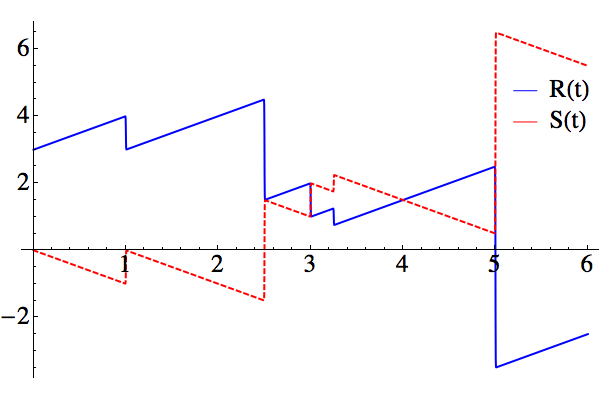
\includegraphics[width=\linewidth]{RiskReserveProcess}
			\caption{\'Evolution des processus de richesse et d'excédent de sinistres au cours du temps.}
				\label{RiskReserveProcessGraphic}
	\end{figureth}
La Figure \ref{RiskReserveProcessGraphic} offre une visualisation graphique de l'évolution des processus de richesse et d'excédent de sinistres. Cette modélisation est dynamique par opposition à la modélisation statique présentée dans les Sections \ref{Chapter1Section1} et \ref{Chapter1Section2}. En théorie de la ruine, l'objectif est d'évaluer la probabilité que le processus de richesse passe en dessous de $0$, en fonction de son point de départ $u$. Cette situation correspond à un situation critique dans laquelle la compagnie n'est plus en mesure de remplir ses engagements vis-à-vis de ses clients, de ses actionnaires ou d'une autorité de contrôle. 
\begin{Def}\label{RuinProbabilityDefinition}
La probabilité de ruine à horizon de temps fini $T$, de réserve initiale $u$ est définie par 
\begin{equation}\label{FiniteTimeRuinProbability}
\psi(u,T)=\mathbb{P}\left(\underset{t\in[0,T]}{\inf}\hspace{0.1cm}R_{t}<0|R_{0}=u\right).
\end{equation}
La probabilité \eqref{FiniteTimeRuinProbability} correspond à la probabilité que les réserves deviennent strictement négatives à un instant précédant l'horizon $T$. La probabilité de ruine ultime ou à horizon de temps infini est définie par  
\begin{equation}\label{UltimateRuinProbability}
\psi(u)=\mathbb{P}\left(\underset{t\geq0}{\inf}\hspace{0.1cm}R_{t}<0|R_{0}=u\right).
\end{equation}
L'instant où la réserve passe en dessous de $0$ coïncide avec l'instant où le processus d'excédent de sinistres passe au-dessus de $u$, cette remarque permet une définition alternative des probabilités de ruine avec
\begin{equation}
\psi(u,T)=\mathbb{P}\left(\underset{t\in[0,T]}{\sup}\hspace{0.1cm}S_{t}>u|S_{0}=0\right), \nonumber
\end{equation}
et
\begin{equation}
\psi(u)=\mathbb{P}\left(\underset{t\geq0}{\sup}\hspace{0.1cm}S_{t}>u|S_{0}=0\right). \nonumber
\end{equation}
La probabilité de non-ruine est définie à horizon de temps fini et infini par 
\begin{equation}
\phi(u,T)=1-\psi(u,T) \nonumber,
\end{equation}
et
\begin{equation}
\phi(u)=1-\psi(u). \nonumber
\end{equation}
\end{Def}
Pour une revue exhaustive des résultats de la  théorie de la ruine, le lecteur peut se référer par exemple aux ouvrages de \citet{Gr91}, \citet{RoScScTe99}, et \citet{AsAl10}.\\ 

Il convient d\rq{}insister sur le caractère extrêmement simplifié du modèle \ref{RiskReserveProcess}, la probabilité de ruine calculée dans le cadre de ce modèle s\rq{}envisage comme une mesure de risque qui va permettre de juger de la pertinence de la tarification de l\rq{}assureur ou encore du niveau de fonds propres à allouer au vue de la sinistralité. Le modèle \ref{RiskReserveProcess} fait office de base à l\rq{}élaboration de modèles plus complexes qui incorporent des taux d\rq{}inflation, une prise en compte de l\rq{}évolution de la sinistralité ou du niveau des primes périodiques. L\rq{}étude des modèles de ruine est aussi rendue interessantes par leur lien avec d\rq{}autres champs d\rq{}application des probabilités. En effet, les modèles de ruine tels que le Modèle \ref{RiskReserveProcess} apparaissent dans d\rq{}autres domaines d\rq{}application des probabilités que l\rq{}actuariat. La théorie des files d\rq{}attente étudie les solutions optimales de gestion des files d\rq{}attente créées par l\rq{}accumulation de clients à des guichets. L\rq{}équivalent du Modèle \ref{RiskReserveProcess} en théorie des files d\rq{}attente est noté $M/G/1$.  Le \lq\lq{}M\rq\rq{} indique que l\rq{}arrivée des clients est gouvernée par un processus ponctuel (Markovien), le \lq\lq{}G\rq\rq{} indique que les temps d\rq{}occupation du guichet par les clients forment une suite de variables aléatoires réelles, positives, et \gls{iid} suivant une loi de probabilité qui n\rq{}est pas spécifiée (Générale), et le \lq\lq{}$1$\rq\rq{} indique que la file d\rq{}attente modélise l\rq{}arrivée des clients sur un seul guichet. La théorie des files d\rq{}attente s\rq{}intéresse à des quantités telles que le temps nécessaire au traitement de toutes les demandes en attente ou encore le temps d\rq{}attente du client $n$. Historiquement, ces modèles ont été introduits pour étudier l\rq{}accumulation de l\rq{}eau retenue par des barrages. L\rq{}utilisation actuelle est plutôt l\rq{}optimisation de la gestion du temps de traitement des données par des serveurs informatiques, pour plus de détails voir le livre d\rq{}\citet{As03}. Récemment, les modèles de ruine et de files d\rq{}attente ont été employés dans l\rq{}étude de l\rq{}évolution de la quantité de contaminants alimentaires présents dans l\rq{}organisme. Le modèle en question a été baptisé \gls{kdem}. L\rq{}ingestion de contaminants par un individu est un évènement supposé ponctuel et aléatoire, l\rq{}arrivée des contaminants dans l\rq{}organisme est par conséquent modélisée via un processus stochastique de comptage. L\rq{}augmentation de la quantité de contaminants dans le corps à chaque ingestion est aléatoire et modélisée par une variable aléatoire réelle, et continue. L\rq{}accumulation de contaminants est un phénomène identique à l\rq{}arrivée de clients à un guichet comme l\rq{}explique le papier de \citet{BeClTr08}. Une fonction d\rq{}élimination des contaminants au cours du temps est définie, et il en résulte un processus de contamination alimentaire dont l\rq{}évolution est inverse à celle de la richesse d\rq{}une compagnie d\rq{}assurance suivant le modèle \ref{RiskReserveProcess}, voir \citet{BeLo14}.\\

Le travail effectué dans cette thèse se focalise sur l'évaluation de la probabilité de ruine ultime \eqref{UltimateRuinProbability} dans un cas particulier du modèle de ruine \ref{ReserveProcess}, appelé modèle de ruine de Poisson composé. Dans le cadre de ce modèle, le processus d'arrivée des sinistres est un processus de Poisson simple d'intensité $\lambda$. Le calcul des probabilités de ruine s'effectue à niveau de prime périodique fixé. L'importance de ce paramètre est à nuancer. La probabilité de ruine est une quantité réaliste lorsqu'elle est faible. Les probabilités de ruine calculées sont associées à des niveaux de réserves initiales très importants relativement au niveau des primes. Le niveau des primes $c$ est contraint par le marché de l'assurance fortement concurrentiel. Une prime périodique élevée entraînerait mécaniquement la fuite des assurés vers les compagnies d'assurance moins chères. Il semble tout de même logique de prélever aux assurés un peu plus que ce qu'ils seront indemnisé en moyenne afin d'avoir une activité rentable. Dans le modèle de ruine de Poisson composé, les assurés coûtent en moyenne
\begin{equation}\label{MeanCost}
\underset{t\rightarrow+\infty}{\lim}\frac{1}{t}\sum_{i=1}^{N_{t}}U_{i}=\lambda E(U),
\end{equation}
par unité de temps. La limite \eqref{MeanCost} est une conséquence de la loi des grands nombres. Le niveau de prime est donné par 
\begin{equation}\label{PremiumLevel}
c=(1+\eta)\lambda\mathbb{E}(U),
\end{equation}   
où $\eta$ est généralement exprimé en pourcentage, et indique de combien la prime doit excéder le coût moyen des sinistres par unité de temps. Une activité rentable est caractérisée par la condition $\eta>0$, appelée \textit{Net Benefit Condition}, et justifiée par le résultat suivant: 
\begin{Prop}\label{PropNetBenefitCondition}
Si $\eta>0$, alors 
\begin{equation}
\underset{t\rightarrow+\infty}{\lim}R_{t}=+\infty,
\end{equation}
$\psi(u)<1$ et l'activité est dite rentable. Si $\eta<0$, alors 
\begin{equation}
\underset{t\rightarrow+\infty}{\lim}R_{t}=-\infty,
\end{equation}
$\psi(u)=1$ et l'activité n'est pas rentable.
\end{Prop}
Il existe un lien entre les distributions composées et la probabilité de ruine ultime dans le modèle de Poisson composé qui se matérialise à travers la \textit{formule de Pollaczek-Khinchine}.
\begin{Theo}[Pollaczek $\&$ Khinchine]\label{PollaczeckKhinchineTheo}
Dans le modèle de ruine de Poisson composé, la probabilité de ruine ultime est égale à la \gls{fds} d'une distribution géométrique composée $(\mathbb{P}_{N},\mathbb{P}_{V})$. Soit $X=\underset{t\geq0}{\sup}\hspace{0.1cm}S_{t}$ alors
\begin{equation}\label{RuinProbabilityGeometricCompoundSurvivalFunction}
\psi(u)=\mathbb{P}(X>u)=(1-p)\sum_{i=1}^{+\infty}p^{i}\overline{F}_{V}^{(*n)}(u),
\end{equation}
avec
\begin{equation}\label{RuinProbabilityGeometricCompoundRV}
X=\sum_{i=1}^{N}V_{i},
\end{equation}
où $N$ est une variable aléatoire de comptage de loi géométrique $\mathcal{NB}(1,p)$ de paramètre $p=\frac{\lambda \mathbb{E}(U)}{c}$, et $\{V_{i}\}_{i\in\mathbb{N}}$ est une suite de variables aléatoires, positives, \gls{iid} suivant une loi $\mathbb{P}_{V}$ et indépendantes de $N$. La distribution de probabilité $\,\mathbb{P}_{V}$ est appelée \textit{integrated tail distribution} de la distribution $\mathbb{P}_{U}$. La densité de probabilité de $\mathbb{P}_{V}$ est donnée par  
\begin{equation}\label{IntegratedTailDistribution}
f_{V}(x)=\frac{\overline{F}_{U}(x)}{\mathbb{E}(U)}.
\end{equation}
La transformée de Laplace de la probabilité de ruine est la transformée de Laplace de la \gls{fds} de la variable aléatoire \eqref{RuinProbabilityGeometricCompoundRV}, soit
\begin{equation}\label{RuinProbabilityLaplaceTransform}
\mathcal{L}_{\psi}(s)=\frac{1}{s}\left(\mathcal{L}_{X}(s)-1\right),
\end{equation}
avec
\begin{equation}\label{LaplaceTransformGeometricCompound}
\mathcal{L}_{X}(s)=\frac{1-p}{1-p\mathcal{L}_{V}(s)},
\end{equation}
et 
\begin{equation}\label{LaplaceTransformIntegratedTailDistribution}
\mathcal{L}_{V}(s)=\frac{1}{s\mathbb{E}(U)}\left(\mathcal{L}_{U}(s)-1\right).
\end{equation}
\end{Theo} 
La présence de la série infinie dans la \textit{formule de Pollaczek-Khinchine} \eqref{RuinProbabilityGeometricCompoundSurvivalFunction} la rend difficilement exploitable pour procéder au calcul de la probabilité de ruine ultime. Celle-ci admet une formule fermée dans un nombre très restreint de cas particuliers, la plupart étant englobés par le résultat suivant. 
\begin{Theo}\label{RuinProbabilityPhaseTypeTheo}
Si le montant des sinistres est distribué suivant une loi de probabilité \textit{phase-type} $\mathcal{PT}(E,\alpha,\bold{T})$, alors
\begin{equation}\label{RuinProbabilityPhaseType}
\psi(u)=\alpha_{+}\exp\left[(\bold{T}+\bold{t}\alpha_{+})u\right],
\end{equation} 
où $\alpha_{+}=-\beta\alpha\bold{T}^{-1}$.
\end{Theo}
Ce résultat est démontré dans le chapitre $8$ du livre d\rq{}\citet{AsAl10}. AInsi, une formule fermée est disponible pour calculer la probabilité de ruine ultime dans le modèle de ruine de Poisson composé lorsque les sinistres sont distribués suivant une loi \textit{phase-type}. 
\begin{Def}
Soit $X$ une variable aléatoire de loi \textit{phase-type} $\mathcal{PT}(E,\alpha,\bold{T})$. $X$ représente le temps d'absorption d'un processus de Markov absorbant d'espace d'état $E$, de générateur $\bold{T}$, et de loi initiale $\alpha$. La densité de $X$ est donnée par 
\begin{equation}\label{DensityPhaseType}
f_{X}(x)=\alpha e^{\bold{T}x}\bold{t},\hspace{0.2cm}x\in\mathbb{R}_{+},
\end{equation}
et sa \gls{fgm} par 
\begin{equation}\label{fgmPhaseType}
\mathcal{L}_{X}(s)=\alpha\left(-s\bold{I}-\bold{T}\right)^{-1}\bold{t},
\end{equation}
où $\bold{I}$ est la matrice identité et $\bold{t}$ vérifie $\bold{t}=\bold{T}\bold{e}$, avec $\bold{e}=(1,\ldots,1)$.
\end{Def}
Un résultat fondamental en théorie de la ruine est l\rq{}encadrement de la probabilité de ruine par des fonctions exponentielles décroissantes. Ce résultat fondamental découle du Théorème \ref{GeometricCoumpoundSurvivalFunctionBoundTheorem}, relatif aux distributions géométriques composées.
\begin{Theo}\label{GeometricCoumpoundSurvivalFunctionBoundTheorem}
Si $X$ admet une distribution géométrique composée $\left[\mathcal{NB}(1,p), \mathbb{P}_{U}\right]$ telle que l'équation
\begin{equation}\label{LundbergEquation1}
\mathcal{L}_{U}(s)=\frac{1}{p}
\end{equation}
admette une unique solution positive, notée $\gamma$, alors 
\begin{equation}\label{GeometricCoumpoundSurvivalFunctionBoundEquation}
a_{-}e^{-\gamma x}<\overline{F}_{X}(x)<a_{+}e^{-\gamma x},
\end{equation}
avec 
\begin{equation}
a_{-}=\underset{x\in\text{Supp}\hspace{0.05cm}U}{\inf}\frac{e^{\gamma x}\overline{F}_{U}(x)}{\int_{x}^{+\infty}e^{\gamma x}\overline{F}_{U}(x)dx},\hspace{1cm} a_{-}=\underset{x\in\text{Supp}\hspace{0.05cm}U}{\sup}\frac{e^{\gamma x}\overline{F}_{U}(x)}{\int_{x}^{+\infty}e^{\gamma x}\overline{F}_{U}(x)dx}.
\end{equation}
\end{Theo}
Une démonstration du Théorème \ref{GeometricCoumpoundSurvivalFunctionBoundTheorem} est donnée au chapitre $4$ de l'ouvrage de \citet{RoScScTe99}. L'application du Théorème \ref{GeometricCoumpoundSurvivalFunctionBoundTheorem} permet d\rq{}établir le résultat suivant:
\begin{Cor}\label{CRamerLundbergBoundRuinProbability}
Dans le modèle de ruine de Poisson composé, la probabilité de ruine vérifie 
\begin{equation}\label{RuinProbabilityBoundEquation}
a_{-}e^{-\gamma u}<\psi(u)<a_{+}e^{-\gamma u},
\end{equation}
où
\begin{equation}
a_{-}=\underset{x\in\text{Supp}\hspace{0.05cm}V}{\inf}\frac{e^{\gamma x}\overline{F}_{V}(x)}{\int_{x}^{+\infty}e^{\gamma x}\overline{F}_{V}(x)dx},\hspace{1cm} a_{-}=\underset{x\in\text{Supp}\hspace{0.05cm}V}{\sup}\frac{e^{\gamma x}\overline{F}_{V}(x)}{\int_{x}^{+\infty}e^{\gamma x}\overline{F}_{V}(x)dx}.
\end{equation}
et $\gamma$ est l'unique solution positive de l'équation
\begin{equation}\label{CramerLunddbergFondamentalEquation}
\lambda\left(\mathcal{L}_{U}(s)-1\right)=cs,
\end{equation}
appelée équation fondamentale de Cramer-Lundberg. 
\end{Cor}
L'existence d'une solution $\gamma>0$ pour l'équation \eqref{CramerLunddbergFondamentalEquation} implique que la \gls{fgm} de la variable aléatoire $U$ est définie sur $[0,\gamma]$. Ce résultat n\rq{}est pas valable si la \gls{fgm} de $U$ n\rq{}est pas définie lorsqu\rq{}elle prend en argument des valeurs positives. Cette situation est typique d'une modélisation du montant des sinistres via une loi de probabilité à queue lourde. Les distributions \textit{phase-type} sont d'ailleurs des distributions de probabilité à queue légère. Le travail effectué ici, se focalise sur l'approximation de la probabilité de ruine lorsque les montants de sinistres sont modélisés par des lois de probabilité à queue légère associées à des transformées de Laplace bien définies. Il s\rq{}agit d\rq{}une condition nécessaire à l\rq{}application des méthodes numériques d\rq{}inversion de la transformée de Laplace. 
\subsection{Approximation de la probabilité de ruine ultime: Revue de la litterature}
Le constat selon lequel la probabilité de ruine ultime n'est accessible que dans un nombre de cas restreint motive la mise au point de méthodes numériques pour l'évaluer. La première approximation proposée est celle de \textit{Cramer-Lundberg}, elle est directement inspirée de l\rq{}encadrement \eqref{RuinProbabilityBoundEquation}. La probabilité de ruine ultime est approchée par
\begin{equation}\label{CramerLundbergApproximation}
\psi(u)=\frac{c-\mathbb{E}(U)}{\lambda\mathcal{L}_{U}(\gamma)-c}e^{-\gamma u}.
\end{equation}
Elle se déduit de l'étude de la limite
\begin{equation}
\underset{u\rightarrow+\infty}{\lim} e^{\gamma u}\psi(u)=\frac{c-\mathbb{E}(U)}{\lambda\mathcal{L}_{U}(\gamma)-c}.
\end{equation}
Elle est performante pour les grandes valeurs de réserves initiales.\\

L'idée de \citet{Bo66} d'approcher la densité de probabilité par des sommes de densités gamma a inspiré le travail de \citet{Be69}, duquel a résulté l'\textit{approximation de Beekman-Bowers} pour la probabilité de ruine ultime. Cette approximation consiste à approcher la loi de probabilité de la variable aléatoire $Z$ dont la loi est caractérisée par sa \gls{fdr}
\begin{equation*}
F_{Z}(u)=1-\frac{\psi(u)}{p},
\end{equation*}
par une loi gamma $\Gamma(\alpha,\beta)$. 
\begin{Def}\label{DefinitionGamma}
Soit $X$ une variable aléatoire de loi gamma $\Gamma(\alpha,\beta)$, de paramètre de forme $\alpha$ et de paramètre d'échellle $\beta$. La densité de la variable aléatoire $X$ est donnée par 
\begin{equation}\label{GammaDensity}
f_{X}(x)=\frac{e^{-x/\beta}x^{\alpha-1}}{\Gamma(\alpha)\beta^{\alpha}},\hspace{0.2cm}x\in\mathbb{R}^{+},
\end{equation}
et sa \gls{fgm} par
\begin{equation}\label{fgmGamma}
\mathcal{L}_{X}(s)=\left(\frac{1}{1-s\beta}\right)^{\alpha}.
\end{equation}
A noter que le cas particulier $\alpha\in\mathbb{N}$ correspond à la loi de Erlang et que le cas très particulier $\alpha=1$ correspond à la loi exponentielle.
\end{Def}
L'identification des paramètres fait coïncider les moments d'ordre $1$ et $2$ de la loi gamma avec ceux de la variable aléatoire $Z$.\\

Le Théorème \ref{RuinProbabilityPhaseTypeTheo} indique que la probabilité de ruine ultime est donnée explicitement par \eqref{RuinProbabilityPhaseType} lorsque le montant des sinistres est distribué suivant une loi \textit{phase-type}. La loi exponentielle est un cas particulier des lois \textit{phase type}, la probabilité de ruine ultime lorsque le montant des sinistres suit une loi exponentielle admet une formule fermée. L'approximation de \citet{DV78} consiste à définir un nouveau processus de réserve financière avec une loi exponentielle $\Gamma(1,\beta)$ pour modéliser la sévérité des sinistres. L'identification des paramètres du nouveau processus de richesse, à savoir l\rq{}intensité du processus de Poisson, le niveau de prime périodique, et le paramètre $\beta$ de la loi du montant des sinistres assure la correspondance des trois premiers moments du nouveau processus de ruine avec ceux de l'ancien. La probabilité de ruine est approchée par la probabilité de ruine ultime associée au nouveau processus de réserve par la formule \eqref{RuinProbabilityPhaseType}. Le papier de \citet{Gr00} propose une étude comparative dans laquelle l\rq{}approximation de \citet{DV78} se distingue de ses concurentes.\\ 

En effet, l'idée sous-tendue par cette approche est le remplacement de la loi pour le montant de sinistres par une loi permettant le calcul de la probabilité de ruine via une formule fermée. Cette idée a inspiré bon nombre de méthodes d'approximation. Les distributions \textit{phase-type} englobent beaucoup de lois de probabilité à support dans $\mathbb{R}^{+}$ comme les mélanges de lois exponentielles et de Erlang. La procédure de \citet{DV78} est utilisée, en prenant comme substitut à la loi de probabilité du montant des sinistres, un mélange de lois exponentielles à deux composantes ou une Erlang de paramètre de forme $\alpha=2$ dans le papier de \citet{Ra92} et une loi gamma plus générale dans le papier de \citet{BuMiWe05}. Cette idée a été approfondie dans le travail de \citet{AvChHo11}. La loi de probabilité du montant des sinistres est approchée par un mélange fini de lois exponentielles. Les paramètres du mélange s'obtiennent en résolvant un système d'équation, dont la complexité est fonction du nombre de composantes dans le mélange. La résolution du système est facilitée par l'utilisation d'une approximation de Padé pour la \gls{fgm} de la variable aléatoire $U$ sous la forme d'une fonction fractionnelle. Une fois les paramètres identifiés, la loi du montant des sinistres est remplacée par la loi issue du mélange fini de lois exponentielles et la probabilité de ruine ultime est approchée par la formule \eqref{RuinProbabilityPhaseType}. Cette méthode est intéréssante car il s'agit d'une procédure d'inversion de la transformée de Laplace basée sur l'étude des moments de la distribution.\\

Le Théorème \ref{PollaczeckKhinchineTheo} rend possible l'application de l'algorithme de Panjer, car la loi géométrique est un cas particulier de la loi binomiale négative qui appartient à la famille de Panjer. La mise en application de l'algorithme de Panjer pour approcher la probabilité de ruine est effectuée dans le papier de \citet{Di95}. D'autres récursions proches de la version continue de l'algorithme de Panjer sont étudiées dans les papiers de \citet{Di89} et \citet{GoVy84}. L'expression de la transformée de Laplace de la probabilité de ruine \eqref{RuinProbabilityLaplaceTransform} permet l'application de l'algorithme \gls{fft}, voir \citet{EmGrPi93}. L'algorithme de Panjer et l'algorithme \gls{fft} admettent les mêmes limites dans l'approximation de la probabilité de ruine ultime que dans le cas des distributions composées. Les méthodes d'inversion numérique de la transformée de Laplace évoquées dans la Section \ref{Chapter1Section1Subsection4} ont aussi été utilisées dans la litterature pour approcher la probabilité de ruine ultime.  La méthode des moments exponentiels est appliquée dans l\rq{}article de \citet{MnSaHa14} et celle des moments fractionels dans le papier de \citet{GzNITa13}. La méthode d'inversion numérique de la transformée de Fourier est appliquée dans le chapitre $5$ du livre de \citet{RoScScTe99}. Récemment, \citet{AlAvKo10} ont proposé une méthode d'inversion qui repose sur une quadrature fondée sur l'approximation rationelle de la fonction exponentielle dans le plan complexe.\\ 

L'application de la méthode basée sur la représentation polynomiale à l'approximation de la probabilité de ruine fait l'objet du papier \citet{GoLoPo15a} et constitue le Chapitre \ref{Chapter4} de ce manuscrit. Ce travail comprend une comparaison avec la méthode d'inversion de la transformée de Fourier, la méthode des moments exponentiels, et l'algorithme de Panjer. La méthode repose sur la combinaison de la loi gamma et des polynômes de Laguerre généralisés. Elle peut être vue comme le prolongement des travaux de \citet{Bo66} et \citet{Be69}. La méthode polynomiale peut aussi être reliée aux travaux de \citet{Ta78} et de \citet{AlTeTi01}, dans lesquels il est supposé que la densité de probabilité gouvernant le montant des sinistres admet un développement sous la forme d'une série infinie de densité gamma. Ce développement est valide si la densité de probabilité est analytique. L'objectif affiché par ces travaux était cependant d'obtenir des formules fermées pour la probabilité de ruine à horizon de temps fini et infini. Ces probabilités admettent aussi des développements en série de densité gamma dont les coefficients sont liés aux développements de la densité de probabilité des montants de sinistre. Des relations de récurrence sont obtenues après réinjection du développement de la densité du montant de sinistres dans les équations vérifiées par la probabilité de ruine. L'exploitation de ces relations de récurrence conduisent dans certains cas à des formules fermées. A noter \citet{Ta78} traite du modèle de ruine de Poisson composé alors que \citet{AlTeTi01} considèrent un modèle de ruine plus général qui comprend un taux d'intérêt, un taux d'inflation et un taux d'actualisation constants. La \textit{formule de Picard-Lefèvre}, voir \citet{PiLe97} et \citet{RuLo04}, donne une formule exacte pour la probabilité de ruine à horizon de temps fini lorsque le montant des sinistres admet une loi discrète. Cette formule est basée sur l\rq{}exploitation des propriétés des polynômes d\rq{}Appell.\\

Ce chapitre a présenté les défis que doivent relever les méthodes numériques d\rq{}approximation et en particulier la méthode polynomiale, décrite exhaustivement dans le Chapitre \ref{Chapter2}. Ce chapitre comprend aussi une illustration des performances de la méthode polynomiale sur l\rq{}exemple de la distribution de Poisson composée. Le Chapitre \ref{Chapter4} traite de l\rq{}approximation polynomiale de la probabilité de ruine ultime dans le modèle de ruine de Poisson composé, et le Chapitre \ref{Chapter5} étudie l\rq{}approximation polynomiale de fonctions associées aux distributions composées bivariées.   
%
%***TODO: Ouverture sur l'estimation statistique de la probabilité de ruine via des méthodes basées sur les moments?*******
%\subsection{L'estimation de la probabilité de ruine ultime en ligne de mire}
%



%L'intérêt des méthodes  
% 
%	\begin{tableth}
%		\caption[Légende courte pour l'exemple de tableau]{Un tableau avec une légende tellement longue que ce serait hideux dans la liste des tableaux}
%			\label{tab:exemple}
%		\begin{tabular}{c|c}
%			Coucou	& Au revoir\\
%			\hline
%			maman	& papa
%		\end{tabular}
%	\end{tableth}
%
%	\begin{figureth}
%		\begin{subfigureth}{0.4\textwidth}
%			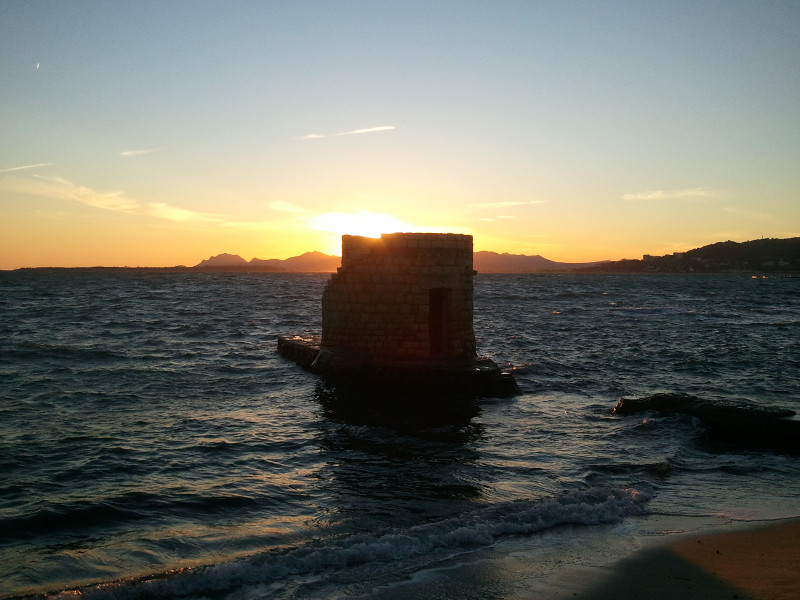
\includegraphics[width=\linewidth]{Antibes}
%			\caption{Photo du Cap d'Antibes}
%				\label{sub:Antibes}
%		\end{subfigureth}
%		\begin{subfigureth}{0.4\textwidth}
%			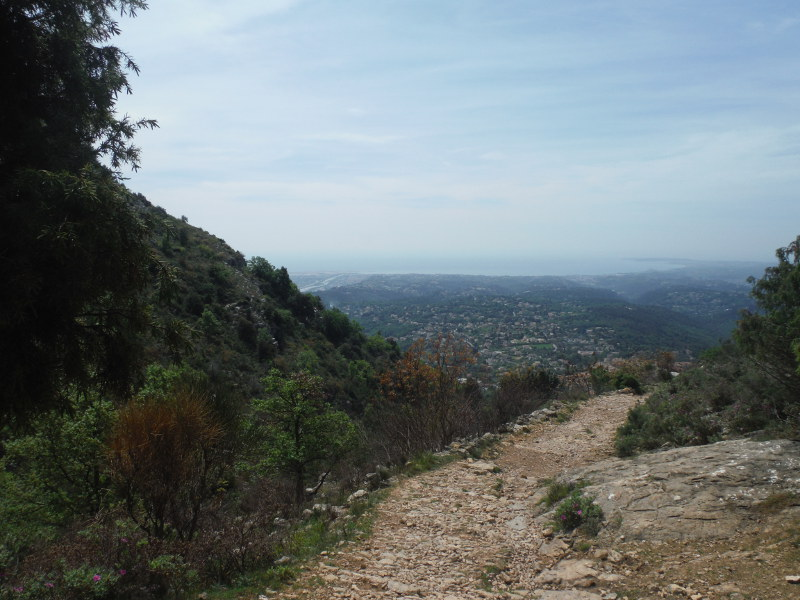
\includegraphics[width=\linewidth]{SaintJeannet}
%			\caption{Saint Jeannet, depuis son Baou}
%				\label{sub:SaintJeannet}
%		\end{subfigureth}
%		\begin{subfigureth}{0.4\textwidth}
%			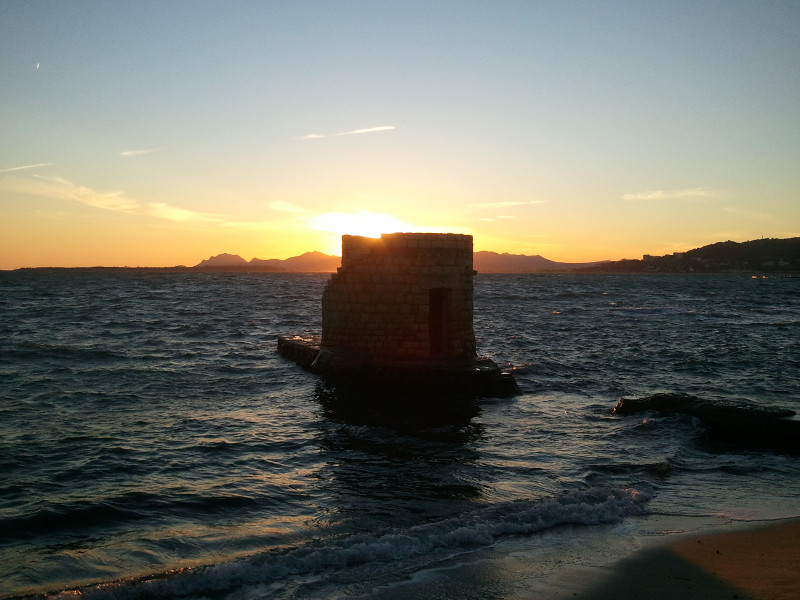
\includegraphics[width=\linewidth]{Antibes}
%			\caption{Photo du Cap d'Antibes}
%				\label{sub:Antibes}
%		\end{subfigureth}
%		\begin{subfigureth}{0.4\textwidth}
%			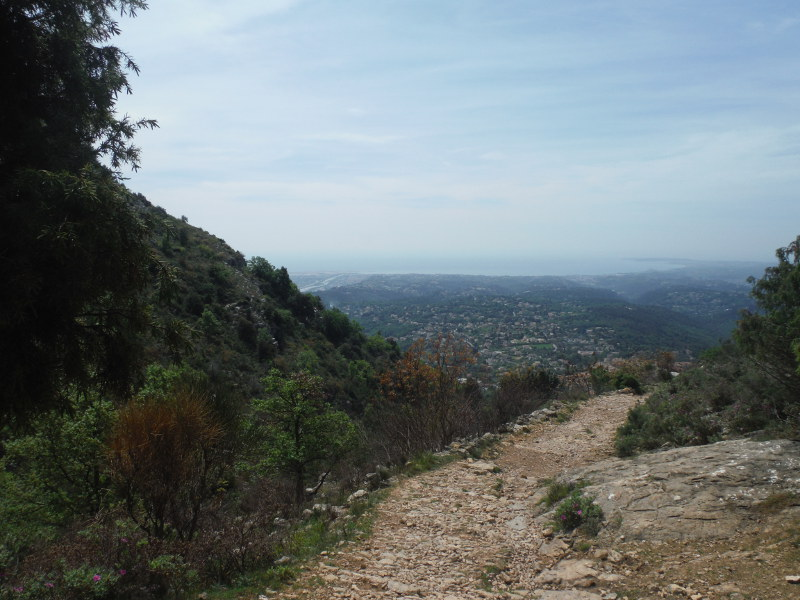
\includegraphics[width=\linewidth]{SaintJeannet}
%			\caption{Saint Jeannet, depuis son Baou}
%				\label{sub:SaintJeannet}
%		\end{subfigureth}
%		\caption[Légende courte pour la figure]{Exemple d'utilisation des sous-figures. J'utilise ici volontairement une légende longue.}		
%			\label{fig:exemple}
%	\end{figureth}
%	
%	\subsection{Symboles mathématiques}
%	Rien de spécial à propos des math, hormis l'illustration des symboles listés en fin de document, tels \gls{alpha} ou \gls{gamma}, qui peuvent être utilisés indifféremment en mode \emph{in-line} ou dans des équations\footnote{Le lecteur notera que \texttt{hyperref} ajoute un lien cliquable sur chaque entrée des différents glossaires.} :
%	\begin{equation}
%		\gls{alpha}=\nicefrac{\gls{gamma}}{2}
%		\label{eq:alphagamma}
%	\end{equation}
%Les entrées des glossaires peuvent même être appelés dans des figures (PDF avec surcouche \LaTeX, ou Ti\textit{k}Z).
%	
%
%\section{Deuxième paragraphe}
%\blindtext

\bibliographystyle{francaissc}
\bibliography{Chapitre1/BiblioChap1}